
% **ATENÇÃO** não editar este arquivo!
%
% o conteúdo deste arquivo é gerado pelo script bin/softwares-summary e pelo
% template capitulos/softwares-summary.tex.epl

\xchapter{Análise de dados dos softwares acadêmicos}{Este capítulo ...}
\label{softwares-summary}

\section{2LS - 2nd order Logic Solving}
\checkmark download
\checkmark código fonte
\checkmark licença


\begin{table}[H]
\caption{Versões lançadas e número de citações ao 2LS por ano}
\centering
\begin{tabular}{| l | c | c | c | c | c |}
  \hline
  Ano & Versões & Peso da citação & Peso da autoria & Peso final & Sustentabilidade técnica \\
  \hline
            {\bf 2015}
          &
          4
          &
          1.00
          &
          0.00
          &
          1.00
          &
            {\color{blue} 1.00}
          \\
\hline
        2016 & 2 & - & - & -
        &
          {\color{blue} 1.00}
        \\
\hline
        2017 & 1 & - & - & -
        &
          {\color{blue} 1.00}
        \\
\hline
\end{tabular}
\end{table}

\begin{figure}[h]
  \center
  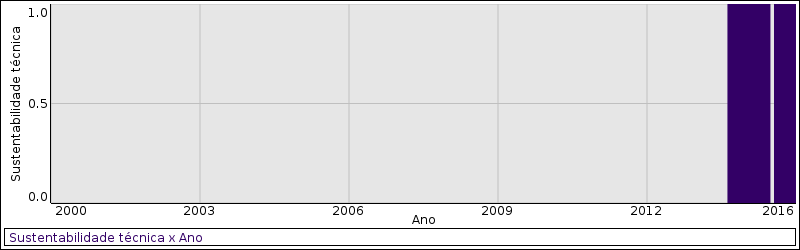
\includegraphics[scale=0.50]{imagens/softwares-charts/2ls.png}
  \caption{Sustentabilidade técnica do 2LS}
\end{figure}


\section{AccessAnalysis}
\checkmark download
\checkmark código fonte
\checkmark licença


\begin{table}[H]
\caption{Versões lançadas e número de citações ao AccessAnalysis por ano}
\centering
\begin{tabular}{| l | c | c | c | c | c |}
  \hline
  Ano & Versões & Peso da citação & Peso da autoria & Peso final & Sustentabilidade técnica \\
  \hline
        2010 & 1 & - & - & -
        &
          {\color{blue} 1.00}
        \\
\hline
            {\bf 2012}
          &
          3
          &
          1.00
          &
          0.00
          &
          1.00
          &
            {\color{blue} 1.00}
          \\
            2012
          &
          
          &
          0.10
          &
          0.00
          &
          0.10
          &
          \\
\hline
\end{tabular}
\end{table}

\begin{figure}[h]
  \center
  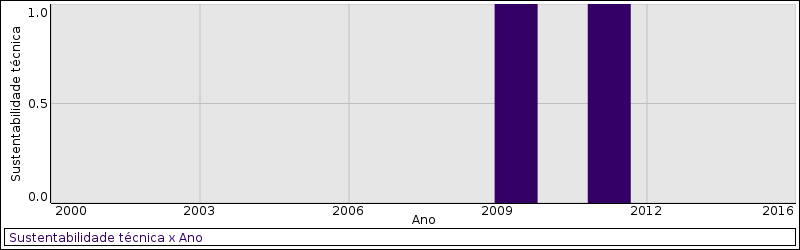
\includegraphics[scale=0.50]{imagens/softwares-charts/accessanalysis.png}
  \caption{Sustentabilidade técnica do AccessAnalysis}
\end{figure}


\section{APIExample}


\begin{table}[H]
\caption{Versões lançadas e número de citações ao APIExample por ano}
\centering
\begin{tabular}{| l | c | c | c | c | c |}
  \hline
  Ano & Versões & Peso da citação & Peso da autoria & Peso final & Sustentabilidade técnica \\
  \hline
            {\bf 2011}
          &
          
          &
          1.00
          &
          0.00
          &
          1.00
          &
            {\color{blue} 1.00}
          \\
\hline
            2013
          &
          
          &
          0.10
          &
          0.25
          &
          0.12
          &
            {\color{red} 0.12}
          \\
            2013
          &
          
          &
          0.10
          &
          0.25
          &
          0.12
          &
          \\
\hline
            2016
          &
          
          &
          0.10
          &
          0.50
          &
          0.15
          &
            {\color{red} 0.15}
          \\
\hline
\end{tabular}
\end{table}

\begin{figure}[h]
  \center
  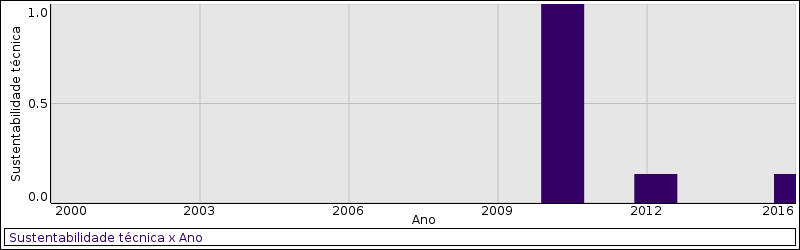
\includegraphics[scale=0.50]{imagens/softwares-charts/apiexample.png}
  \caption{Sustentabilidade técnica do APIExample}
\end{figure}


\section{BEG - Bandera environment generator}


\begin{table}[H]
\caption{Versões lançadas e número de citações ao BEG por ano}
\centering
\begin{tabular}{| l | c | c | c | c | c |}
  \hline
  Ano & Versões & Peso da citação & Peso da autoria & Peso final & Sustentabilidade técnica \\
  \hline
            {\bf 2003}
          &
          
          &
          1.00
          &
          0.00
          &
          1.00
          &
            {\color{blue} 1.00}
          \\
\hline
            2004
          &
          
          &
          0.25
          &
          0.25
          &
          0.31
          &
            {\color{red} 0.31}
          \\
\hline
            2006
          &
          
          &
          0.25
          &
          0.25
          &
          0.31
          &
            {\color{red} 0.31}
          \\
            2006
          &
          
          &
          0.10
          &
          0.25
          &
          0.12
          &
          \\
\hline
            2007
          &
          
          &
          0.25
          &
          0.10
          &
          0.28
          &
            {\color{red} 0.28}
          \\
            2007
          &
          
          &
          0.10
          &
          0.25
          &
          0.12
          &
          \\
\hline
            2010
          &
          
          &
          0.10
          &
          0.10
          &
          0.11
          &
            {\color{blue} 0.55}
          \\
            2010
          &
          
          &
          0.50
          &
          0.10
          &
          0.55
          &
          \\
\hline
            2015
          &
          
          &
          0.10
          &
          0.50
          &
          0.15
          &
            {\color{red} 0.15}
          \\
\hline
\end{tabular}
\end{table}

\begin{figure}[h]
  \center
  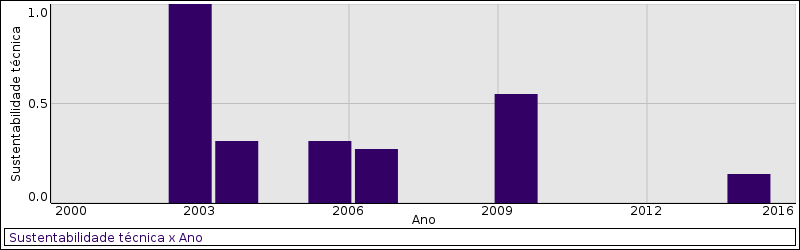
\includegraphics[scale=0.50]{imagens/softwares-charts/beg.png}
  \caption{Sustentabilidade técnica do BEG}
\end{figure}


\section{ccJava - Class-based Crosscutting Language for Java}


\begin{table}[H]
\caption{Versões lançadas e número de citações ao ccJava por ano}
\centering
\begin{tabular}{| l | c | c | c | c | c |}
  \hline
  Ano & Versões & Peso da citação & Peso da autoria & Peso final & Sustentabilidade técnica \\
  \hline
            {\bf 2007}
          &
          
          &
          1.00
          &
          0.00
          &
          1.00
          &
            {\color{blue} 1.00}
          \\
            2007
          &
          
          &
          0.10
          &
          0.00
          &
          0.10
          &
          \\
\hline
            2008
          &
          
          &
          0.50
          &
          0.00
          &
          0.50
          &
            {\color{blue} 0.50}
          \\
\hline
            2009
          &
          
          &
          0.50
          &
          0.25
          &
          0.62
          &
            {\color{blue} 0.62}
          \\
\hline
            2010
          &
          
          &
          0.50
          &
          0.10
          &
          0.55
          &
            {\color{blue} 0.55}
          \\
\hline
\end{tabular}
\end{table}

\begin{figure}[h]
  \center
  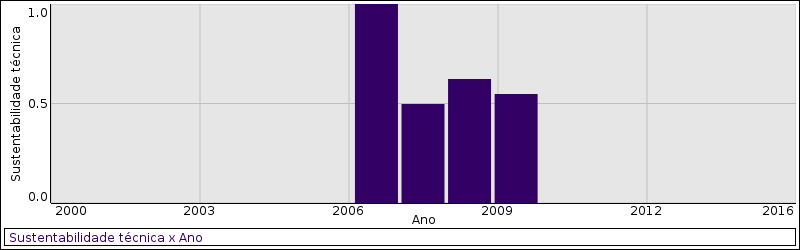
\includegraphics[scale=0.50]{imagens/softwares-charts/ccjava.png}
  \caption{Sustentabilidade técnica do ccJava}
\end{figure}


\section{CIVL - Concurrency intermediate verification language}
\checkmark download
\checkmark código fonte
\checkmark licença


\begin{table}[H]
\caption{Versões lançadas e número de citações ao CIVL por ano}
\centering
\begin{tabular}{| l | c | c | c | c | c |}
  \hline
  Ano & Versões & Peso da citação & Peso da autoria & Peso final & Sustentabilidade técnica \\
  \hline
            2015
          &
          25
          &
          0.10
          &
          0.00
          &
          0.10
          &
            {\color{blue} 1.00}
          \\
            {\bf 2015}
          &
          
          &
          1.00
          &
          0.00
          &
          1.00
          &
          \\
            2015
          &
          
          &
          0.10
          &
          0.00
          &
          0.10
          &
          \\
            2015
          &
          
          &
          0.10
          &
          0.00
          &
          0.10
          &
          \\
\hline
        2016 & 5 & - & - & -
        &
          {\color{blue} 1.00}
        \\
\hline
            2017
          &
          6
          &
          0.10
          &
          0.25
          &
          0.12
          &
            {\color{blue} 1.00}
          \\
            2017
          &
          
          &
          0.10
          &
          0.25
          &
          0.12
          &
          \\
\hline
\end{tabular}
\end{table}

\begin{figure}[h]
  \center
  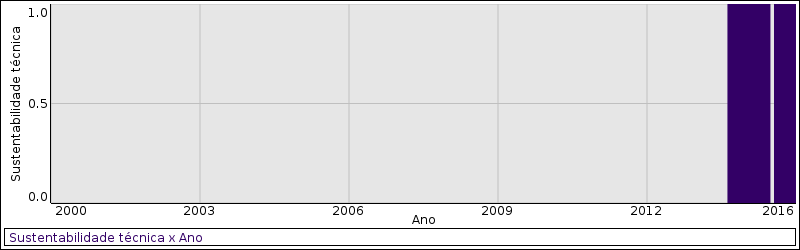
\includegraphics[scale=0.50]{imagens/softwares-charts/civl.png}
  \caption{Sustentabilidade técnica do CIVL}
\end{figure}


\section{CodeBoost}
\checkmark download
\checkmark código fonte
\checkmark licença


\begin{table}[H]
\caption{Versões lançadas e número de citações ao CodeBoost por ano}
\centering
\begin{tabular}{| l | c | c | c | c | c |}
  \hline
  Ano & Versões & Peso da citação & Peso da autoria & Peso final & Sustentabilidade técnica \\
  \hline
        2000 & 36 & - & - & -
        &
          {\color{blue} 1.00}
        \\
\hline
        2001 & 35 & - & - & -
        &
          {\color{blue} 1.00}
        \\
\hline
        2002 & 49 & - & - & -
        &
          {\color{blue} 1.00}
        \\
\hline
            {\bf 2003}
          &
          8
          &
          1.00
          &
          0.00
          &
          1.00
          &
            {\color{blue} 1.00}
          \\
            2003
          &
          
          &
          0.10
          &
          0.00
          &
          0.10
          &
          \\
\hline
        2004 & 6 & - & - & -
        &
          {\color{blue} 1.00}
        \\
\hline
            2005
          &
          
          &
          0.10
          &
          0.25
          &
          0.12
          &
            {\color{red} 0.12}
          \\
            2005
          &
          
          &
          0.10
          &
          0.10
          &
          0.11
          &
          \\
            2005
          &
          
          &
          0.10
          &
          0.25
          &
          0.12
          &
          \\
\hline
            2006
          &
          
          &
          0.10
          &
          0.25
          &
          0.12
          &
            {\color{red} 0.12}
          \\
            2006
          &
          
          &
          0.10
          &
          0.25
          &
          0.12
          &
          \\
\hline
            2008
          &
          
          &
          0.10
          &
          0.50
          &
          0.15
          &
            {\color{red} 0.15}
          \\
\hline
            2009
          &
          
          &
          0.10
          &
          0.25
          &
          0.12
          &
            {\color{red} 0.12}
          \\
\hline
            2010
          &
          
          &
          0.10
          &
          0.50
          &
          0.15
          &
            {\color{red} 0.15}
          \\
\hline
            2011
          &
          
          &
          0.10
          &
          0.50
          &
          0.15
          &
            {\color{red} 0.15}
          \\
            2011
          &
          
          &
          0.10
          &
          0.50
          &
          0.15
          &
          \\
\hline
            2012
          &
          
          &
          0.10
          &
          0.25
          &
          0.12
          &
            {\color{red} 0.12}
          \\
\hline
            2013
          &
          
          &
          0.10
          &
          0.50
          &
          0.15
          &
            {\color{red} 0.15}
          \\
\hline
            2015
          &
          
          &
          0.10
          &
          0.50
          &
          0.15
          &
            {\color{red} 0.15}
          \\
\hline
\end{tabular}
\end{table}

\begin{figure}[h]
  \center
  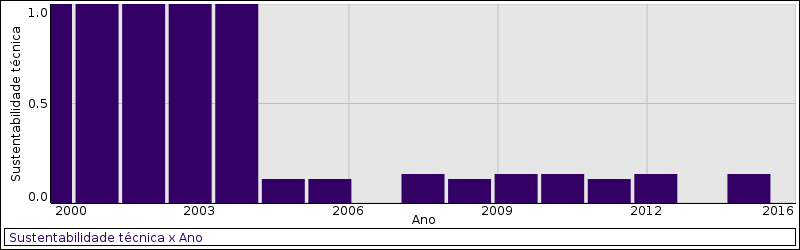
\includegraphics[scale=0.50]{imagens/softwares-charts/codeboost.png}
  \caption{Sustentabilidade técnica do CodeBoost}
\end{figure}


\section{CSL - Composite Symbolic Library}
\checkmark download
\checkmark código fonte


\begin{table}[H]
\caption{Versões lançadas e número de citações ao CSL por ano}
\centering
\begin{tabular}{| l | c | c | c | c | c |}
  \hline
  Ano & Versões & Peso da citação & Peso da autoria & Peso final & Sustentabilidade técnica \\
  \hline
            {\bf 2001}
          &
          
          &
          1.00
          &
          0.00
          &
          1.00
          &
            {\color{blue} 1.00}
          \\
\hline
            2004
          &
          
          &
          0.10
          &
          0.25
          &
          0.12
          &
            {\color{red} 0.12}
          \\
\hline
            2005
          &
          
          &
          0.10
          &
          0.50
          &
          0.15
          &
            {\color{red} 0.15}
          \\
\hline
            2006
          &
          
          &
          0.10
          &
          0.25
          &
          0.12
          &
            {\color{blue} 0.75}
          \\
            2006
          &
          
          &
          0.50
          &
          0.50
          &
          0.75
          &
          \\
\hline
            2009
          &
          
          &
          0.25
          &
          0.25
          &
          0.31
          &
            {\color{red} 0.31}
          \\
\hline
\end{tabular}
\end{table}

\begin{figure}[h]
  \center
  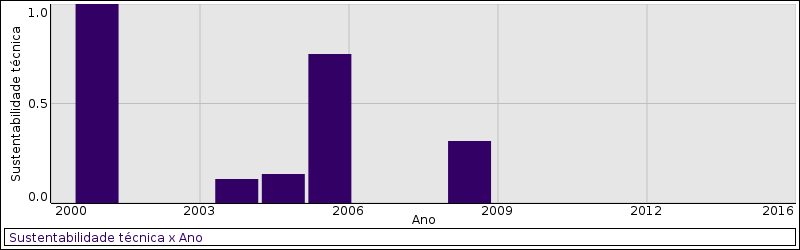
\includegraphics[scale=0.50]{imagens/softwares-charts/composite.png}
  \caption{Sustentabilidade técnica do CSL}
\end{figure}


\section{CPA+ - Configurable program analysis with dynamic precision adjustment}


\begin{table}[H]
\caption{Versões lançadas e número de citações ao CPA+ por ano}
\centering
\begin{tabular}{| l | c | c | c | c | c |}
  \hline
  Ano & Versões & Peso da citação & Peso da autoria & Peso final & Sustentabilidade técnica \\
  \hline
            {\bf 2008}
          &
          
          &
          1.00
          &
          0.00
          &
          1.00
          &
            {\color{blue} 1.00}
          \\
\hline
            2010
          &
          
          &
          0.50
          &
          0.25
          &
          0.62
          &
            {\color{blue} 0.62}
          \\
\hline
            2012
          &
          
          &
          0.50
          &
          0.10
          &
          0.55
          &
            {\color{blue} 0.55}
          \\
\hline
            2013
          &
          
          &
          0.50
            {\tiny CPA+ = CPAchecker}
          &
          0.25
          &
          0.62
          &
            {\color{blue} 0.62}
          \\
\hline
            2015
          &
          
          &
          0.50
          &
          0.25
          &
          0.62
          &
            {\color{blue} 0.62}
          \\
\hline
\end{tabular}
\end{table}

\begin{figure}[h]
  \center
  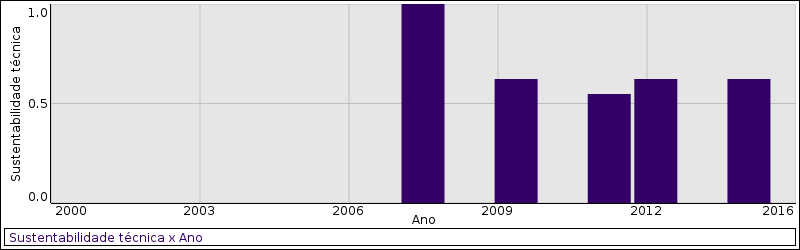
\includegraphics[scale=0.50]{imagens/softwares-charts/cpa+.png}
  \caption{Sustentabilidade técnica do CPA+}
\end{figure}


\section{CSeq}
\checkmark download
\checkmark código fonte
\checkmark licença


\begin{table}[H]
\caption{Versões lançadas e número de citações ao CSeq por ano}
\centering
\begin{tabular}{| l | c | c | c | c | c |}
  \hline
  Ano & Versões & Peso da citação & Peso da autoria & Peso final & Sustentabilidade técnica \\
  \hline
            {\bf 2013}
          &
          
          &
          1.00
          &
          0.00
          &
          1.00
          &
            {\color{blue} 1.00}
          \\
\hline
            2015
          &
          
          &
          0.50
          &
          0.00
          &
          0.50
          &
            {\color{blue} 0.50}
          \\
            2015
          &
          
          &
          0.25
          &
          0.00
          &
          0.25
          &
          \\
\hline
            2016
          &
          
          &
          0.10
          &
          0.50
          &
          0.15
          &
            {\color{red} 0.31}
          \\
            2016
          &
          
          &
          0.25
          &
          0.25
          &
          0.31
          &
          \\
\hline
\end{tabular}
\end{table}

\begin{figure}[h]
  \center
  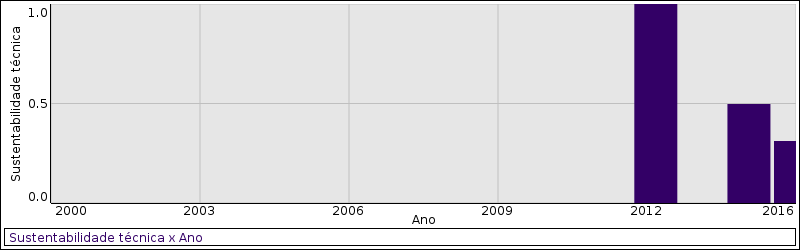
\includegraphics[scale=0.50]{imagens/softwares-charts/cseq.png}
  \caption{Sustentabilidade técnica do CSeq}
\end{figure}


\section{DDVerify}


\begin{table}[H]
\caption{Versões lançadas e número de citações ao DDVerify por ano}
\centering
\begin{tabular}{| l | c | c | c | c | c |}
  \hline
  Ano & Versões & Peso da citação & Peso da autoria & Peso final & Sustentabilidade técnica \\
  \hline
            {\bf 2007}
          &
          
          &
          1.00
          &
          0.00
          &
          1.00
          &
            {\color{blue} 1.00}
          \\
\hline
            2008
          &
          
          &
          0.10
          &
          0.10
          &
          0.11
          &
            {\color{red} 0.11}
          \\
\hline
            2014
          &
          
          &
          0.10
          &
          0.50
          &
          0.15
          &
            {\color{red} 0.15}
          \\
\hline
\end{tabular}
\end{table}

\begin{figure}[h]
  \center
  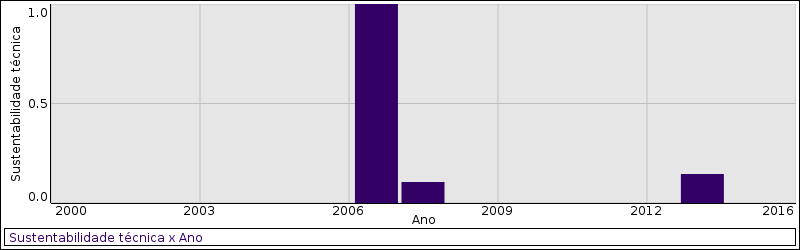
\includegraphics[scale=0.50]{imagens/softwares-charts/ddverify.png}
  \caption{Sustentabilidade técnica do DDVerify}
\end{figure}


\section{Derailer}
\checkmark download
\checkmark código fonte
\checkmark licença


\begin{table}[H]
\caption{Versões lançadas e número de citações ao Derailer por ano}
\centering
\begin{tabular}{| l | c | c | c | c | c |}
  \hline
  Ano & Versões & Peso da citação & Peso da autoria & Peso final & Sustentabilidade técnica \\
  \hline
        2013 & 1 & - & - & -
        &
          {\color{blue} 1.00}
        \\
\hline
            {\bf 2014}
          &
          1
          &
          1.00
          &
          0.00
          &
          1.00
          &
            {\color{blue} 1.00}
          \\
\hline
            2016
          &
          
          &
          0.10
            {\tiny SPACE}
          &
          0.10
          &
          0.11
          &
            {\color{red} 0.11}
          \\
\hline
\end{tabular}
\end{table}

\begin{figure}[h]
  \center
  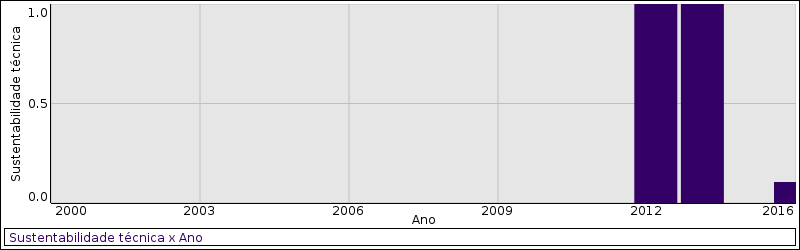
\includegraphics[scale=0.50]{imagens/softwares-charts/derailer.png}
  \caption{Sustentabilidade técnica do Derailer}
\end{figure}


\section{Diagnosys}


\begin{table}[H]
\caption{Versões lançadas e número de citações ao Diagnosys por ano}
\centering
\begin{tabular}{| l | c | c | c | c | c |}
  \hline
  Ano & Versões & Peso da citação & Peso da autoria & Peso final & Sustentabilidade técnica \\
  \hline
            {\bf 2012}
          &
          
          &
          1.00
          &
          0.00
          &
          1.00
          &
            {\color{blue} 1.00}
          \\
\hline
\end{tabular}
\end{table}

\begin{figure}[h]
  \center
  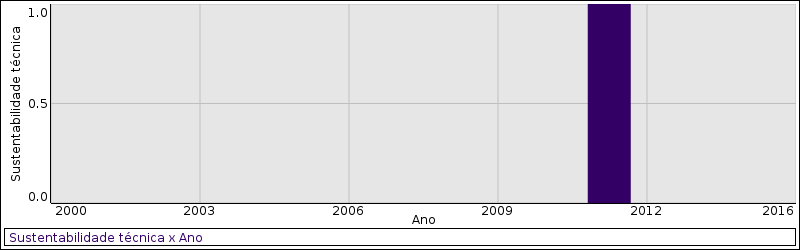
\includegraphics[scale=0.50]{imagens/softwares-charts/diagnosys.png}
  \caption{Sustentabilidade técnica do Diagnosys}
\end{figure}


\section{DOMPLETION}
\checkmark download
\checkmark código fonte


\begin{table}[H]
\caption{Versões lançadas e número de citações ao DOMPLETION por ano}
\centering
\begin{tabular}{| l | c | c | c | c | c |}
  \hline
  Ano & Versões & Peso da citação & Peso da autoria & Peso final & Sustentabilidade técnica \\
  \hline
            {\bf 2014}
          &
          
          &
          1.00
          &
          0.00
          &
          1.00
          &
            {\color{blue} 1.00}
          \\
\hline
            2015
          &
          
          &
          0.10
          &
          0.10
          &
          0.11
          &
            {\color{red} 0.11}
          \\
\hline
\end{tabular}
\end{table}

\begin{figure}[h]
  \center
  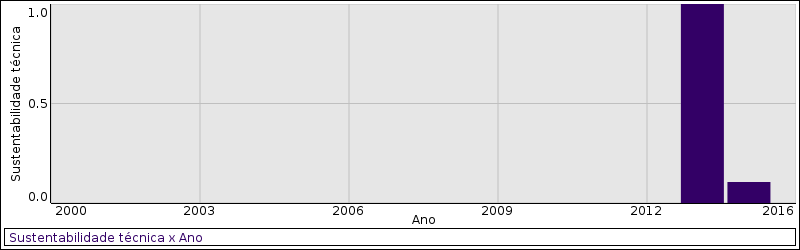
\includegraphics[scale=0.50]{imagens/softwares-charts/dompletion.png}
  \caption{Sustentabilidade técnica do DOMPLETION}
\end{figure}


\section{DRC - Dangling Reference Checker}


\begin{table}[H]
\caption{Versões lançadas e número de citações ao DRC por ano}
\centering
\begin{tabular}{| l | c | c | c | c | c |}
  \hline
  Ano & Versões & Peso da citação & Peso da autoria & Peso final & Sustentabilidade técnica \\
  \hline
            2013
          &
          
          &
          0.10
          &
          0.00
          &
          0.10
          &
            {\color{blue} 1.00}
          \\
            {\bf 2013}
          &
          
          &
          1.00
          &
          0.00
          &
          1.00
          &
          \\
\hline
            2014
          &
          
          &
          0.10
          &
          0.25
          &
          0.12
          &
            {\color{red} 0.15}
          \\
            2014
          &
          
          &
          0.10
          &
          0.50
          &
          0.15
          &
          \\
\hline
            2015
          &
          
          &
          0.10
          &
          0.10
          &
          0.11
          &
            {\color{red} 0.11}
          \\
\hline
\end{tabular}
\end{table}

\begin{figure}[h]
  \center
  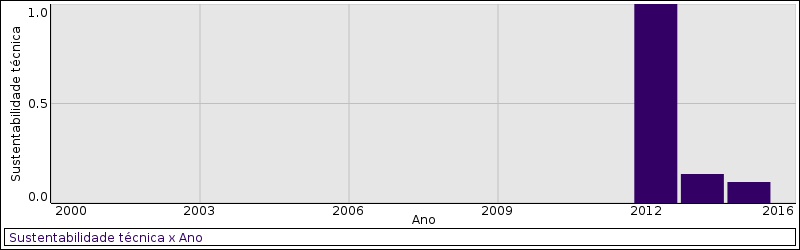
\includegraphics[scale=0.50]{imagens/softwares-charts/drc.png}
  \caption{Sustentabilidade técnica do DRC}
\end{figure}


\section{e-munity}
\checkmark download
\checkmark código fonte


\begin{table}[H]
\caption{Versões lançadas e número de citações ao e-munity por ano}
\centering
\begin{tabular}{| l | c | c | c | c | c |}
  \hline
  Ano & Versões & Peso da citação & Peso da autoria & Peso final & Sustentabilidade técnica \\
  \hline
            {\bf 2014}
          &
          
          &
          1.00
          &
          0.00
          &
          1.00
          &
            {\color{blue} 1.00}
          \\
\hline
\end{tabular}
\end{table}

\begin{figure}[h]
  \center
  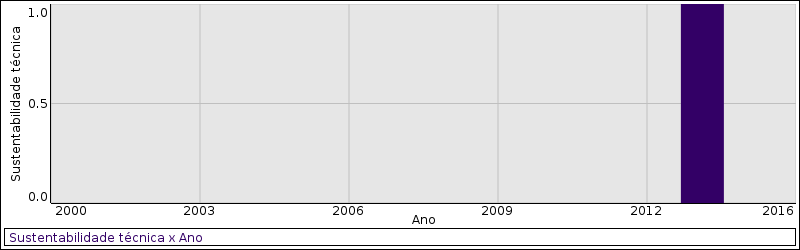
\includegraphics[scale=0.50]{imagens/softwares-charts/e-munity.png}
  \caption{Sustentabilidade técnica do e-munity}
\end{figure}


\section{EJB Interceptor Analyzer}
\checkmark download
\checkmark código fonte


\begin{table}[H]
\caption{Versões lançadas e número de citações ao EJB Interceptor Analyzer por ano}
\centering
\begin{tabular}{| l | c | c | c | c | c |}
  \hline
  Ano & Versões & Peso da citação & Peso da autoria & Peso final & Sustentabilidade técnica \\
  \hline
            {\bf 2011}
          &
          
          &
          1.00
          &
          0.00
          &
          1.00
          &
            {\color{blue} 1.00}
          \\
\hline
            2013
          &
          
          &
          0.10
            {\tiny I2SD = EJB}
          &
          0.25
          &
          0.12
          &
            {\color{red} 0.12}
          \\
\hline
            2017
          &
          
          &
          0.25
          &
          0.50
          &
          0.38
          &
            {\color{red} 0.38}
          \\
\hline
\end{tabular}
\end{table}

\begin{figure}[h]
  \center
  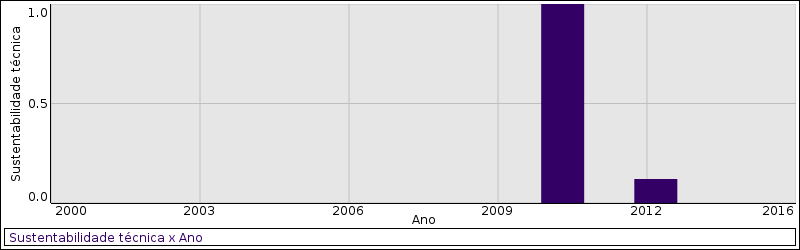
\includegraphics[scale=0.50]{imagens/softwares-charts/ejb.png}
  \caption{Sustentabilidade técnica do EJB Interceptor Analyzer}
\end{figure}


\section{Error Prone}
\checkmark download
\checkmark código fonte
\checkmark licença


\begin{table}[H]
\caption{Versões lançadas e número de citações ao Error Prone por ano}
\centering
\begin{tabular}{| l | c | c | c | c | c |}
  \hline
  Ano & Versões & Peso da citação & Peso da autoria & Peso final & Sustentabilidade técnica \\
  \hline
            {\bf 2012}
          &
          
          &
          1.00
          &
          0.00
          &
          1.00
          &
            {\color{blue} 1.00}
          \\
\hline
            2015
          &
          8
          &
          0.25
          &
          0.50
          &
          0.38
          &
            {\color{blue} 1.00}
          \\
\hline
        2016 & 8 & - & - & -
        &
          {\color{blue} 1.00}
        \\
\hline
        2017 & 6 & - & - & -
        &
          {\color{blue} 1.00}
        \\
\hline
\end{tabular}
\end{table}

\begin{figure}[h]
  \center
  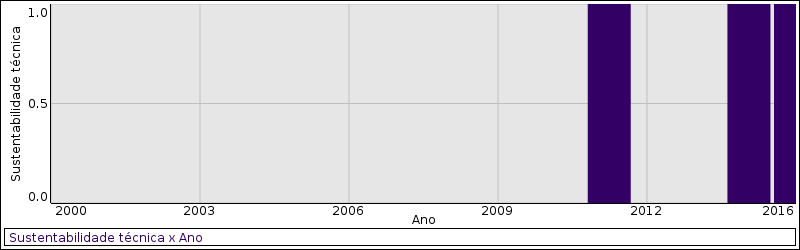
\includegraphics[scale=0.50]{imagens/softwares-charts/error-prone.png}
  \caption{Sustentabilidade técnica do Error Prone}
\end{figure}


\section{ESBMC - Efficient SMT-Based Context-Bounded Model Checker}


\begin{table}[H]
\caption{Versões lançadas e número de citações ao ESBMC por ano}
\centering
\begin{tabular}{| l | c | c | c | c | c |}
  \hline
  Ano & Versões & Peso da citação & Peso da autoria & Peso final & Sustentabilidade técnica \\
  \hline
            {\bf 2009}
          &
          
          &
          1.00
          &
          0.00
          &
          1.00
          &
            {\color{blue} 1.00}
          \\
\hline
            2010
          &
          
          &
          0.25
          &
          0.10
          &
          0.28
          &
            {\color{red} 0.28}
          \\
\hline
            2011
          &
          
          &
          0.25
          &
          0.50
          &
          0.38
          &
            {\color{blue} 0.62}
          \\
            2011
          &
          
          &
          0.50
          &
          0.25
          &
          0.62
          &
          \\
            2011
          &
          
          &
          0.25
          &
          0.25
          &
          0.31
          &
          \\
\hline
            2012
          &
          
          &
          0.25
          &
          0.50
          &
          0.38
          &
            {\color{red} 0.38}
          \\
            2012
          &
          
          &
          0.25
          &
          0.50
          &
          0.38
          &
          \\
\hline
            2013
          &
          
          &
          0.25
          &
          0.25
          &
          0.31
          &
            {\color{blue} 0.62}
          \\
            2013
          &
          
          &
          0.10
          &
          0.25
          &
          0.12
          &
          \\
            2013
          &
          
          &
          0.10
          &
          0.25
          &
          0.12
          &
          \\
            2013
          &
          
          &
          0.50
          &
          0.25
          &
          0.62
          &
          \\
            2013
          &
          
          &
          0.25
          &
          0.25
          &
          0.31
          &
          \\
            2013
          &
          
          &
          0.25
          &
          0.25
          &
          0.31
          &
          \\
\hline
            2014
          &
          
          &
          0.50
          &
          0.25
          &
          0.62
          &
            {\color{blue} 0.62}
          \\
            2014
          &
          
          &
          0.25
          &
          0.25
          &
          0.31
          &
          \\
            2014
          &
          
          &
          0.10
          &
          0.50
          &
          0.15
          &
          \\
            2014
          &
          
          &
          0.25
          &
          0.25
          &
          0.31
          &
          \\
            2014
          &
          
          &
          0.25
          &
          0.25
          &
          0.31
          &
          \\
            2014
          &
          
          &
          0.25
          &
          0.25
          &
          0.31
          &
          \\
\hline
            2015
          &
          
          &
          0.50
          &
          0.25
          &
          0.62
          &
            {\color{blue} 0.62}
          \\
            2015
          &
          
          &
          0.10
          &
          0.25
          &
          0.12
          &
          \\
            2015
          &
          
          &
          0.50
          &
          0.25
          &
          0.62
          &
          \\
            2015
          &
          
          &
          0.25
          &
          0.25
          &
          0.31
          &
          \\
            2015
          &
          
          &
          0.10
          &
          0.25
          &
          0.12
          &
          \\
            2015
          &
          
          &
          0.50
          &
          0.25
          &
          0.62
          &
          \\
            2015
          &
          
          &
          0.25
          &
          0.25
          &
          0.31
          &
          \\
            2015
          &
          
          &
          0.10
          &
          0.25
          &
          0.12
          &
          \\
\hline
            2016
          &
          
          &
          0.25
          &
          0.25
          &
          0.31
          &
            {\color{blue} 0.62}
          \\
            2016
          &
          
          &
          0.10
          &
          0.25
          &
          0.12
          &
          \\
            2016
          &
          
          &
          0.10
          &
          0.50
          &
          0.15
          &
          \\
            2016
          &
          
          &
          0.25
          &
          0.25
          &
          0.31
          &
          \\
            2016
          &
          
          &
          0.10
          &
          0.25
          &
          0.12
          &
          \\
            2016
          &
          
          &
          0.10
          &
          0.25
          &
          0.12
          &
          \\
            2016
          &
          
          &
          0.10
          &
          0.25
          &
          0.12
          &
          \\
            2016
          &
          
          &
          0.10
          &
          0.25
          &
          0.12
          &
          \\
            2016
          &
          
          &
          0.25
          &
          0.25
          &
          0.31
          &
          \\
            2016
          &
          
          &
          0.10
          &
          0.25
          &
          0.12
          &
          \\
            2016
          &
          
          &
          0.50
          &
          0.25
          &
          0.62
          &
          \\
\hline
            2017
          &
          
          &
          0.25
          &
          0.25
          &
          0.31
          &
            {\color{red} 0.31}
          \\
            2017
          &
          
          &
          0.25
          &
          0.25
          &
          0.31
          &
          \\
            2017
          &
          
          &
          0.10
          &
          0.25
          &
          0.12
          &
          \\
            2017
          &
          
          &
          0.10
          &
          0.25
          &
          0.12
          &
          \\
\hline
\end{tabular}
\end{table}

\begin{figure}[h]
  \center
  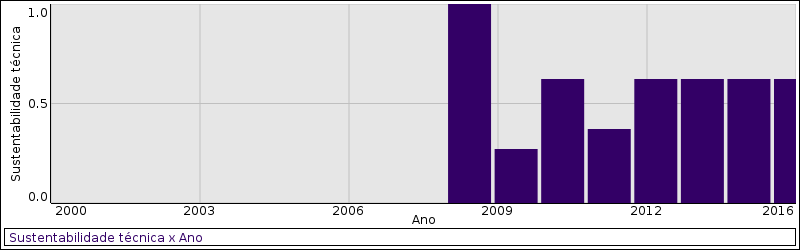
\includegraphics[scale=0.50]{imagens/softwares-charts/esbmc.png}
  \caption{Sustentabilidade técnica do ESBMC}
\end{figure}


\section{ETXL}


\begin{table}[H]
\caption{Versões lançadas e número de citações ao ETXL por ano}
\centering
\begin{tabular}{| l | c | c | c | c | c |}
  \hline
  Ano & Versões & Peso da citação & Peso da autoria & Peso final & Sustentabilidade técnica \\
  \hline
            {\bf 2006}
          &
          
          &
          1.00
          &
          0.00
          &
          1.00
          &
            {\color{blue} 1.00}
          \\
\hline
\end{tabular}
\end{table}

\begin{figure}[h]
  \center
  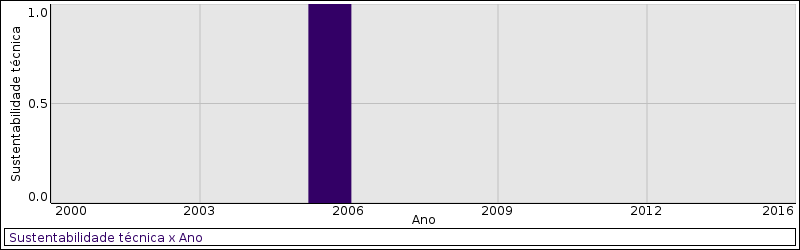
\includegraphics[scale=0.50]{imagens/softwares-charts/etxl.png}
  \caption{Sustentabilidade técnica do ETXL}
\end{figure}


\section{FaultBuster}
\checkmark download
\checkmark licença


\begin{table}[H]
\caption{Versões lançadas e número de citações ao FaultBuster por ano}
\centering
\begin{tabular}{| l | c | c | c | c | c |}
  \hline
  Ano & Versões & Peso da citação & Peso da autoria & Peso final & Sustentabilidade técnica \\
  \hline
            {\bf 2015}
          &
          
          &
          1.00
          &
          0.00
          &
          1.00
          &
            {\color{blue} 1.00}
          \\
\hline
\end{tabular}
\end{table}

\begin{figure}[h]
  \center
  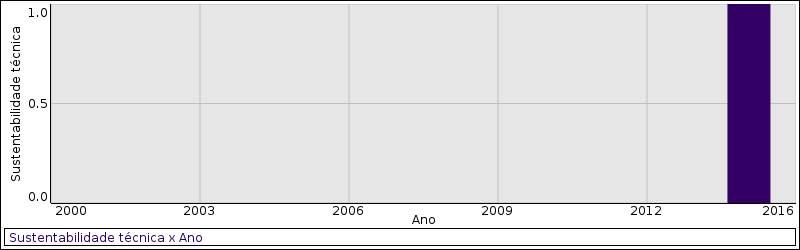
\includegraphics[scale=0.50]{imagens/softwares-charts/faultbuster.png}
  \caption{Sustentabilidade técnica do FaultBuster}
\end{figure}


\section{Flowgen}
\checkmark download
\checkmark código fonte
\checkmark licença


\begin{table}[H]
\caption{Versões lançadas e número de citações ao Flowgen por ano}
\centering
\begin{tabular}{| l | c | c | c | c | c |}
  \hline
  Ano & Versões & Peso da citação & Peso da autoria & Peso final & Sustentabilidade técnica \\
  \hline
            {\bf 2014}
          &
          
          &
          1.00
          &
          0.00
          &
          1.00
          &
            {\color{blue} 1.00}
          \\
\hline
            2015
          &
          
          &
          0.10
          &
          0.50
          &
          0.15
          &
            {\color{red} 0.15}
          \\
\hline
            2016
          &
          
          &
          0.10
          &
          0.50
          &
          0.15
          &
            {\color{red} 0.15}
          \\
\hline
\end{tabular}
\end{table}

\begin{figure}[h]
  \center
  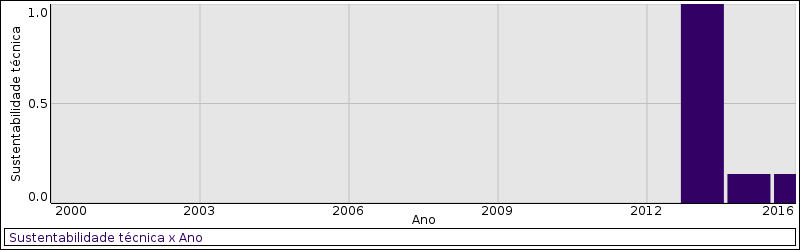
\includegraphics[scale=0.50]{imagens/softwares-charts/flowgen.png}
  \caption{Sustentabilidade técnica do Flowgen}
\end{figure}


\section{GRT - Guided Random Testing}


\begin{table}[H]
\caption{Versões lançadas e número de citações ao GRT por ano}
\centering
\begin{tabular}{| l | c | c | c | c | c |}
  \hline
  Ano & Versões & Peso da citação & Peso da autoria & Peso final & Sustentabilidade técnica \\
  \hline
            2014
          &
          
          &
          0.10
            {\tiny BGRT}
          &
          0.00
          &
          0.10
          &
            {\color{red} 0.10}
          \\
\hline
            2015
          &
          
          &
          0.10
            {\tiny 1º no SBST '15}
          &
          0.50
          &
          0.15
          &
            {\color{blue} 0.75}
          \\
            {\bf 2015}
          &
          
          &
          0.50
          &
          0.50
          &
          0.75
          &
          \\
            {\bf 2015}
          &
          
          &
          0.50
          &
          0.50
          &
          0.75
          &
          \\
\hline
            2016
          &
          
          &
          0.25
          &
          0.10
          &
          0.28
          &
            {\color{blue} 0.62}
          \\
            2016
          &
          
          &
          0.50
          &
          0.25
          &
          0.62
          &
          \\
\hline
            2017
          &
          
          &
          0.10
          &
          0.50
          &
          0.15
          &
            {\color{red} 0.31}
          \\
            2017
          &
          
          &
          0.25
          &
          0.25
          &
          0.31
          &
          \\
            2017
          &
          
          &
          0.10
          &
          0.25
          &
          0.12
          &
          \\
\hline
\end{tabular}
\end{table}

\begin{figure}[h]
  \center
  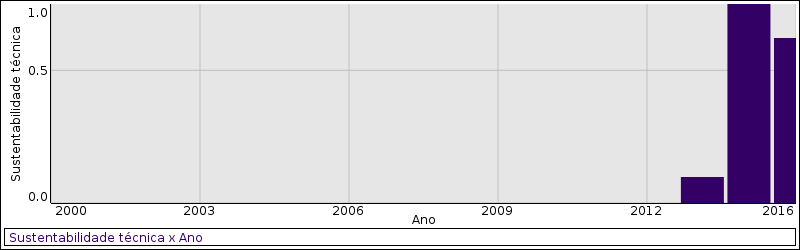
\includegraphics[scale=0.50]{imagens/softwares-charts/grt.png}
  \caption{Sustentabilidade técnica do GRT}
\end{figure}


\section{GUIZMO}
\checkmark download
\checkmark código fonte
\checkmark licença


\begin{table}[H]
\caption{Versões lançadas e número de citações ao GUIZMO por ano}
\centering
\begin{tabular}{| l | c | c | c | c | c |}
  \hline
  Ano & Versões & Peso da citação & Peso da autoria & Peso final & Sustentabilidade técnica \\
  \hline
            {\bf 2010}
          &
          
          &
          1.00
          &
          0.00
          &
          1.00
          &
            {\color{blue} 1.00}
          \\
\hline
\end{tabular}
\end{table}

\begin{figure}[h]
  \center
  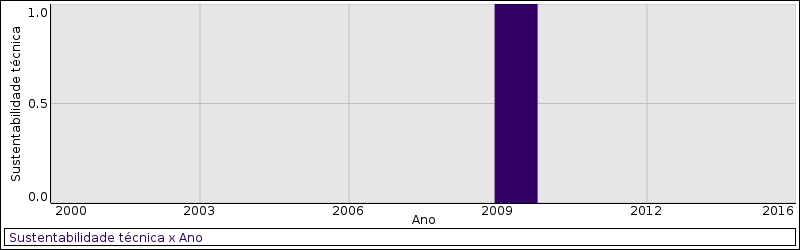
\includegraphics[scale=0.50]{imagens/softwares-charts/guizmo.png}
  \caption{Sustentabilidade técnica do GUIZMO}
\end{figure}


\section{GumTree}
\checkmark download
\checkmark código fonte
\checkmark licença


\begin{table}[H]
\caption{Versões lançadas e número de citações ao GumTree por ano}
\centering
\begin{tabular}{| l | c | c | c | c | c |}
  \hline
  Ano & Versões & Peso da citação & Peso da autoria & Peso final & Sustentabilidade técnica \\
  \hline
        2013 & 1 & - & - & -
        &
          {\color{blue} 1.00}
        \\
\hline
            {\bf 2014}
          &
          
          &
          1.00
          &
          0.00
          &
          1.00
          &
            {\color{blue} 1.00}
          \\
\hline
            2015
          &
          2
          &
          0.10
          &
          0.50
          &
          0.15
          &
            {\color{blue} 1.00}
          \\
            2015
          &
          
          &
          0.25
          &
          0.50
          &
          0.38
          &
          \\
\hline
            2016
          &
          
          &
          0.25
          &
          0.50
          &
          0.38
          &
            {\color{red} 0.38}
          \\
            2016
          &
          
          &
          0.10
          &
          0.50
          &
          0.15
          &
          \\
            2016
          &
          
          &
          0.25
          &
          0.50
          &
          0.38
          &
          \\
            2016
          &
          
          &
          0.25
          &
          0.50
          &
          0.38
          &
          \\
            2016
          &
          
          &
          0.25
          &
          0.50
          &
          0.38
          &
          \\
            2016
          &
          
          &
          0.25
          &
          0.50
          &
          0.38
          &
          \\
\hline
            2017
          &
          
          &
          0.25
          &
          0.25
          &
          0.31
          &
            {\color{blue} 0.62}
          \\
            2017
          &
          
          &
          0.10
          &
          0.25
          &
          0.12
          &
          \\
            2017
          &
          
          &
          0.50
          &
          0.25
          &
          0.62
          &
          \\
            2017
          &
          
          &
          0.10
          &
          0.25
          &
          0.12
          &
          \\
            2017
          &
          
          &
          0.25
          &
          0.25
          &
          0.31
          &
          \\
            2017
          &
          
          &
          0.10
          &
          0.25
          &
          0.12
          &
          \\
            2017
          &
          
          &
          0.25
          &
          0.25
          &
          0.31
          &
          \\
            2017
          &
          
          &
          0.25
          &
          0.25
          &
          0.31
          &
          \\
            2017
          &
          
          &
          0.25
          &
          0.25
          &
          0.31
          &
          \\
\hline
\end{tabular}
\end{table}

\begin{figure}[h]
  \center
  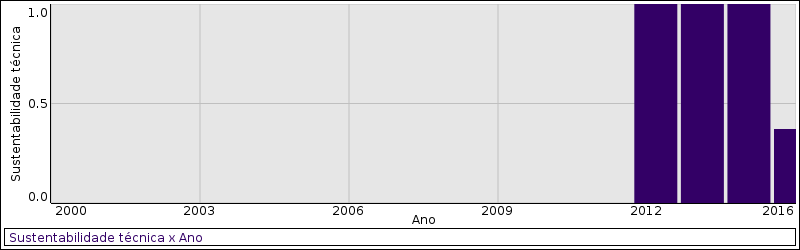
\includegraphics[scale=0.50]{imagens/softwares-charts/gumtree.png}
  \caption{Sustentabilidade técnica do GumTree}
\end{figure}


\section{HUSACCT - HU Software Architecture Compliance Checking Tool}
\checkmark download
\checkmark código fonte
\checkmark licença


\begin{table}[H]
\caption{Versões lançadas e número de citações ao HUSACCT por ano}
\centering
\begin{tabular}{| l | c | c | c | c | c |}
  \hline
  Ano & Versões & Peso da citação & Peso da autoria & Peso final & Sustentabilidade técnica \\
  \hline
        2013 & 3 & - & - & -
        &
          {\color{blue} 1.00}
        \\
\hline
            2014
          &
          7
          &
          0.10
          &
          0.00
          &
          0.10
          &
            {\color{blue} 1.00}
          \\
            {\bf 2014}
          &
          
          &
          1.00
          &
          0.00
          &
          1.00
          &
          \\
\hline
            2015
          &
          6
          &
          0.25
          &
          0.25
          &
          0.31
          &
            {\color{blue} 1.00}
          \\
\hline
            2016
          &
          3
          &
          0.10
          &
          0.25
          &
          0.12
          &
            {\color{blue} 1.00}
          \\
            2016
          &
          
          &
          0.10
          &
          0.25
          &
          0.12
          &
          \\
            2016
          &
          
          &
          1.00
          &
          0.25
          &
          1.00
          &
          \\
            2016
          &
          
          &
          0.25
          &
          0.25
          &
          0.31
          &
          \\
\hline
        2017 & 3 & - & - & -
        &
          {\color{blue} 1.00}
        \\
\hline
\end{tabular}
\end{table}

\begin{figure}[h]
  \center
  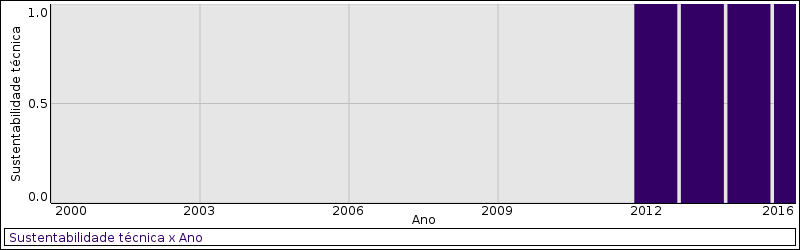
\includegraphics[scale=0.50]{imagens/softwares-charts/husacct.png}
  \caption{Sustentabilidade técnica do HUSACCT}
\end{figure}


\section{Indus}
\checkmark download
\checkmark código fonte
\checkmark licença


\begin{table}[H]
\caption{Versões lançadas e número de citações ao Indus por ano}
\centering
\begin{tabular}{| l | c | c | c | c | c |}
  \hline
  Ano & Versões & Peso da citação & Peso da autoria & Peso final & Sustentabilidade técnica \\
  \hline
        2005 & 13 & - & - & -
        &
          {\color{blue} 1.00}
        \\
\hline
            {\bf 2006}
          &
          14
          &
          1.00
          &
          0.00
          &
          1.00
          &
            {\color{blue} 1.00}
          \\
\hline
        2007 & 6 & - & - & -
        &
          {\color{blue} 1.00}
        \\
\hline
            2009
          &
          2
          &
          0.25
          &
          0.50
          &
          0.38
          &
            {\color{blue} 1.00}
          \\
\hline
        2010 & 1 & - & - & -
        &
          {\color{blue} 1.00}
        \\
\hline
            2012
          &
          
          &
          0.25
          &
          0.25
          &
          0.31
          &
            {\color{red} 0.31}
          \\
            2012
          &
          
          &
          0.25
          &
          0.25
          &
          0.31
          &
          \\
\hline
\end{tabular}
\end{table}

\begin{figure}[h]
  \center
  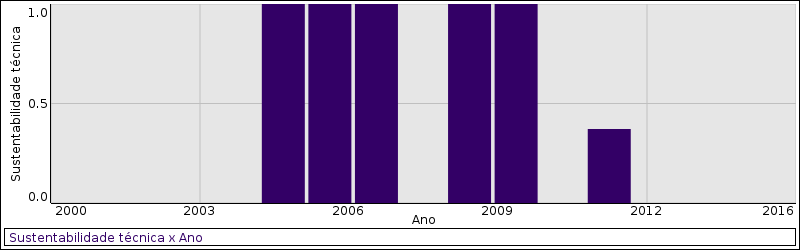
\includegraphics[scale=0.50]{imagens/softwares-charts/indus.png}
  \caption{Sustentabilidade técnica do Indus}
\end{figure}


\section{JastAdd}
\checkmark download
\checkmark código fonte
\checkmark licença


\begin{table}[H]
\caption{Versões lançadas e número de citações ao JastAdd por ano}
\centering
\begin{tabular}{| l | c | c | c | c | c |}
  \hline
  Ano & Versões & Peso da citação & Peso da autoria & Peso final & Sustentabilidade técnica \\
  \hline
            2003
          &
          
          &
          0.10
          &
          0.00
          &
          0.10
          &
            {\color{red} 0.10}
          \\
\hline
            2005
          &
          
          &
          0.10
          &
          0.50
          &
          0.15
          &
            {\color{red} 0.38}
          \\
            2005
          &
          
          &
          0.25
          &
          0.50
          &
          0.38
          &
          \\
            2005
          &
          
          &
          0.10
          &
          0.50
          &
          0.15
          &
          \\
            2005
          &
          
          &
          0.10
          &
          0.50
          &
          0.15
          &
          \\
\hline
            2006
          &
          
          &
          0.10
          &
          0.50
          &
          0.15
          &
            {\color{red} 0.31}
          \\
            2006
          &
          
          &
          0.10
          &
          0.25
          &
          0.12
          &
          \\
            2006
          &
          
          &
          0.25
          &
          0.25
          &
          0.31
          &
          \\
\hline
            2007
          &
          
          &
          0.10
          &
          0.25
          &
          0.12
          &
            {\color{blue} 1.00}
          \\
            {\bf 2007}
          &
          
          &
          1.00
          &
          0.25
          &
          1.00
          &
          \\
            2007
          &
          
          &
          0.25
          &
          0.25
          &
          0.31
          &
          \\
            2007
          &
          
          &
          0.25
          &
          0.25
          &
          0.31
          &
          \\
\hline
            2008
          &
          
          &
          0.10
          &
          0.25
          &
          0.12
          &
            {\color{blue} 0.62}
          \\
            2008
          &
          
          &
          0.10
          &
          0.25
          &
          0.12
          &
          \\
            2008
          &
          
          &
          0.25
          &
          0.25
          &
          0.31
          &
          \\
            2008
          &
          
          &
          0.50
          &
          0.25
          &
          0.62
          &
          \\
\hline
            2009
          &
          
          &
          0.10
          &
          0.25
          &
          0.12
          &
            {\color{red} 0.15}
          \\
            2009
          &
          
          &
          0.10
          &
          0.50
          &
          0.15
          &
          \\
\hline
            2010
          &
          
          &
          0.10
          &
          0.25
          &
          0.12
          &
            {\color{blue} 0.62}
          \\
            2010
          &
          
          &
          0.25
          &
          0.25
          &
          0.31
          &
          \\
            2010
          &
          
          &
          0.10
          &
          0.25
          &
          0.12
          &
          \\
            2010
          &
          
          &
          0.10
          &
          0.25
          &
          0.12
          &
          \\
            2010
          &
          
          &
          0.50
          &
          0.25
          &
          0.62
          &
          \\
            2010
          &
          
          &
          0.10
          &
          0.25
          &
          0.12
          &
          \\
\hline
            2011
          &
          1
          &
          0.25
          &
          0.25
          &
          0.31
          &
            {\color{blue} 1.00}
          \\
            2011
          &
          
          &
          0.10
          &
          0.50
          &
          0.15
          &
          \\
            2011
          &
          
          &
          0.10
          &
          0.50
          &
          0.15
          &
          \\
\hline
            2012
          &
          3
          &
          0.25
          &
          0.25
          &
          0.31
          &
            {\color{blue} 1.00}
          \\
            2012
          &
          
          &
          0.25
          &
          0.25
          &
          0.31
          &
          \\
            2012
          &
          
          &
          0.25
          &
          0.25
          &
          0.31
          &
          \\
            2012
          &
          
          &
          0.10
          &
          0.25
          &
          0.12
          &
          \\
\hline
            2013
          &
          9
          &
          0.25
          &
          0.25
          &
          0.31
          &
            {\color{blue} 1.00}
          \\
            2013
          &
          
          &
          0.25
          &
          0.25
          &
          0.31
          &
          \\
            2013
          &
          
          &
          0.50
          &
          0.25
          &
          0.62
          &
          \\
\hline
            2014
          &
          4
          &
          0.10
          &
          0.25
          &
          0.12
          &
            {\color{blue} 1.00}
          \\
            2014
          &
          
          &
          0.25
          &
          0.10
          &
          0.28
          &
          \\
\hline
            2015
          &
          3
          &
          0.10
          &
          0.25
          &
          0.12
          &
            {\color{blue} 1.00}
          \\
            2015
          &
          
          &
          0.10
          &
          0.25
          &
          0.12
          &
          \\
\hline
            2016
          &
          3
          &
          0.25
          &
          0.25
          &
          0.31
          &
            {\color{blue} 1.00}
          \\
            2016
          &
          
          &
          0.10
          &
          0.25
          &
          0.12
          &
          \\
            2016
          &
          
          &
          0.25
          &
          0.25
          &
          0.31
          &
          \\
\hline
            2017
          &
          1
          &
          0.10
          &
          0.50
          &
          0.15
          &
            {\color{blue} 1.00}
          \\
            2017
          &
          
          &
          0.10
          &
          0.50
          &
          0.15
          &
          \\
\hline
\end{tabular}
\end{table}

\begin{figure}[h]
  \center
  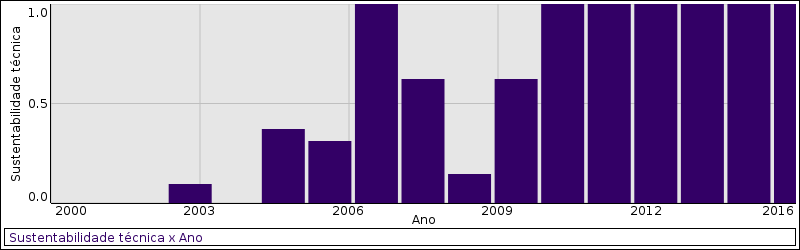
\includegraphics[scale=0.50]{imagens/softwares-charts/jastadd.png}
  \caption{Sustentabilidade técnica do JastAdd}
\end{figure}


\section{JFlow}
\checkmark download
\checkmark código fonte
\checkmark licença


\begin{table}[H]
\caption{Versões lançadas e número de citações ao JFlow por ano}
\centering
\begin{tabular}{| l | c | c | c | c | c |}
  \hline
  Ano & Versões & Peso da citação & Peso da autoria & Peso final & Sustentabilidade técnica \\
  \hline
            2006
          &
          
          &
          0.10
          &
          0.00
          &
          0.10
          &
            {\color{red} 0.10}
          \\
            2006
          &
          
          &
          0.10
          &
          0.00
          &
          0.10
          &
          \\
\hline
            2007
          &
          
          &
          0.25
          &
          0.25
          &
          0.31
          &
            {\color{red} 0.31}
          \\
\hline
            2011
          &
          
          &
          0.10
          &
          0.50
          &
          0.15
          &
            {\color{red} 0.15}
          \\
            2011
          &
          
          &
          0.10
          &
          0.50
          &
          0.15
          &
          \\
\hline
        2012 & 5 & - & - & -
        &
          {\color{blue} 1.00}
        \\
\hline
            {\bf 2013}
          &
          
          &
          1.00
          &
          0.50
          &
          1.00
          &
            {\color{blue} 1.00}
          \\
\hline
            2014
          &
          
          &
          0.10
          &
          0.50
          &
          0.15
          &
            {\color{red} 0.15}
          \\
\hline
\end{tabular}
\end{table}

\begin{figure}[h]
  \center
  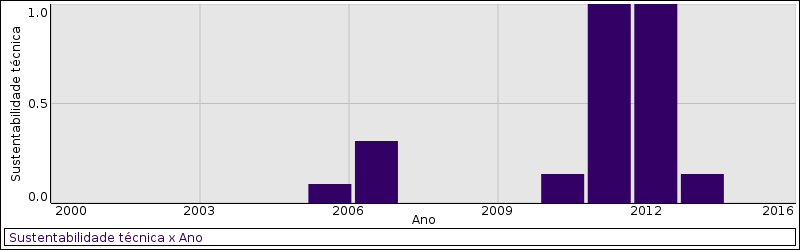
\includegraphics[scale=0.50]{imagens/softwares-charts/jflow.png}
  \caption{Sustentabilidade técnica do JFlow}
\end{figure}


\section{JstereoCode}


\begin{table}[H]
\caption{Versões lançadas e número de citações ao JstereoCode por ano}
\centering
\begin{tabular}{| l | c | c | c | c | c |}
  \hline
  Ano & Versões & Peso da citação & Peso da autoria & Peso final & Sustentabilidade técnica \\
  \hline
            {\bf 2012}
          &
          
          &
          1.00
          &
          0.00
          &
          1.00
          &
            {\color{blue} 1.00}
          \\
\hline
            2013
          &
          
          &
          0.25
          &
          0.00
          &
          0.25
          &
            {\color{red} 0.25}
          \\
            2013
          &
          
          &
          0.25
          &
          0.00
          &
          0.25
          &
          \\
            2013
          &
          
          &
          0.10
          &
          0.00
          &
          0.10
          &
          \\
\hline
            2015
          &
          
          &
          0.25
          &
          0.25
          &
          0.31
          &
            {\color{red} 0.31}
          \\
            2015
          &
          
          &
          0.25
          &
          0.25
          &
          0.31
          &
          \\
\hline
            2016
          &
          
          &
          0.25
          &
          0.50
          &
          0.38
          &
            {\color{red} 0.38}
          \\
\hline
            2017
          &
          
          &
          0.10
          &
          0.50
          &
          0.15
          &
            {\color{red} 0.15}
          \\
\hline
\end{tabular}
\end{table}

\begin{figure}[h]
  \center
  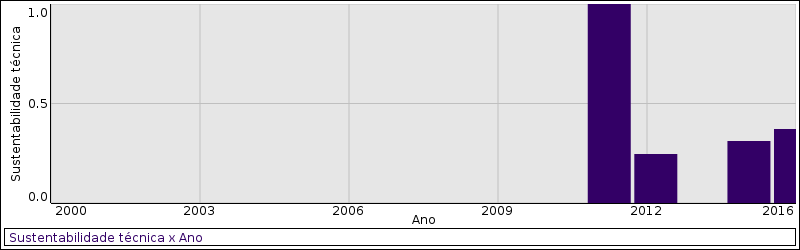
\includegraphics[scale=0.50]{imagens/softwares-charts/jstereocode.png}
  \caption{Sustentabilidade técnica do JstereoCode}
\end{figure}


\section{Jtop}
\checkmark licença


\begin{table}[H]
\caption{Versões lançadas e número de citações ao Jtop por ano}
\centering
\begin{tabular}{| l | c | c | c | c | c |}
  \hline
  Ano & Versões & Peso da citação & Peso da autoria & Peso final & Sustentabilidade técnica \\
  \hline
            {\bf 2009}
          &
          
          &
          1.00
          &
          0.00
          &
          1.00
          &
            {\color{blue} 1.00}
          \\
\hline
            2014
          &
          
          &
          0.25
          &
          0.25
          &
          0.31
          &
            {\color{red} 0.31}
          \\
\hline
\end{tabular}
\end{table}

\begin{figure}[h]
  \center
  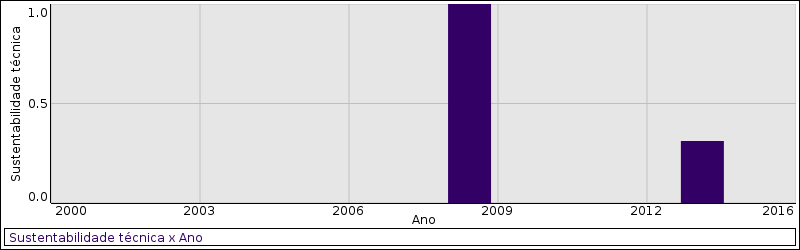
\includegraphics[scale=0.50]{imagens/softwares-charts/jtop.png}
  \caption{Sustentabilidade técnica do Jtop}
\end{figure}


\section{Bogor/Kiasan}
\checkmark download
\checkmark código fonte
\checkmark licença


\begin{table}[H]
\caption{Versões lançadas e número de citações ao Bogor/Kiasan por ano}
\centering
\begin{tabular}{| l | c | c | c | c | c |}
  \hline
  Ano & Versões & Peso da citação & Peso da autoria & Peso final & Sustentabilidade técnica \\
  \hline
            {\bf 2006}
          &
          
          &
          1.00
          &
          0.00
          &
          1.00
          &
            {\color{blue} 1.00}
          \\
            2006
          &
          
          &
          0.50
          &
          0.00
          &
          0.50
          &
          \\
\hline
            2007
          &
          
          &
          0.10
          &
          0.25
          &
          0.12
          &
            {\color{blue} 0.62}
          \\
            2007
          &
          
          &
          0.50
          &
          0.25
          &
          0.62
          &
          \\
            2007
          &
          
          &
          0.50
          &
          0.25
          &
          0.62
          &
          \\
\hline
            2008
          &
          
          &
          0.10
          &
          0.50
          &
          0.15
          &
            {\color{red} 0.15}
          \\
            2008
          &
          
          &
          0.10
          &
          0.50
          &
          0.15
          &
          \\
            2008
          &
          
          &
          0.10
          &
          0.50
          &
          0.15
          &
          \\
\hline
            2009
          &
          
          &
          0.10
          &
          0.25
          &
          0.12
          &
            {\color{blue} 0.62}
          \\
            2009
          &
          
          &
          0.50
          &
          0.25
          &
          0.62
          &
          \\
\hline
            2010
          &
          
          &
          0.10
          &
          0.25
          &
          0.12
          &
            {\color{red} 0.12}
          \\
            2010
          &
          
          &
          0.10
          &
          0.25
          &
          0.12
          &
          \\
            2010
          &
          
          &
          0.10
          &
          0.25
          &
          0.12
          &
          \\
\hline
            2013
          &
          
          &
          0.10
          &
          0.50
          &
          0.15
          &
            {\color{red} 0.15}
          \\
\hline
            2014
          &
          
          &
          0.50
          &
          0.25
          &
          0.62
          &
            {\color{blue} 0.62}
          \\
\hline
            2015
          &
          
          &
          0.10
          &
          0.50
          &
          0.15
          &
            {\color{red} 0.15}
          \\
\hline
\end{tabular}
\end{table}

\begin{figure}[h]
  \center
  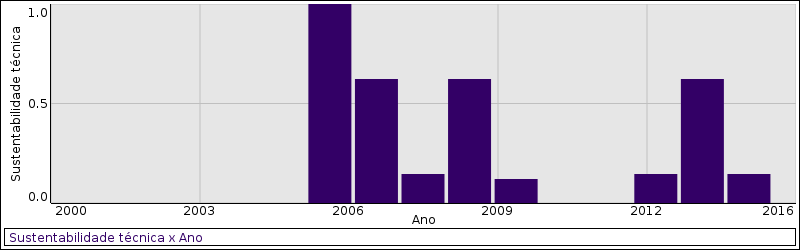
\includegraphics[scale=0.50]{imagens/softwares-charts/kiasan.png}
  \caption{Sustentabilidade técnica do Bogor/Kiasan}
\end{figure}


\section{Loopfrog}
\checkmark download


\begin{table}[H]
\caption{Versões lançadas e número de citações ao Loopfrog por ano}
\centering
\begin{tabular}{| l | c | c | c | c | c |}
  \hline
  Ano & Versões & Peso da citação & Peso da autoria & Peso final & Sustentabilidade técnica \\
  \hline
            {\bf 2009}
          &
          
          &
          1.00
          &
          0.00
          &
          1.00
          &
            {\color{blue} 1.00}
          \\
\hline
            2012
          &
          
          &
          0.10
          &
          0.50
          &
          0.15
          &
            {\color{red} 0.15}
          \\
\hline
            2013
          &
          
          &
          0.10
          &
          0.50
          &
          0.15
          &
            {\color{red} 0.38}
          \\
            2013
          &
          
          &
          0.25
          &
          0.50
          &
          0.38
          &
          \\
            2013
          &
          
          &
          0.25
          &
          0.50
          &
          0.38
          &
          \\
\hline
\end{tabular}
\end{table}

\begin{figure}[h]
  \center
  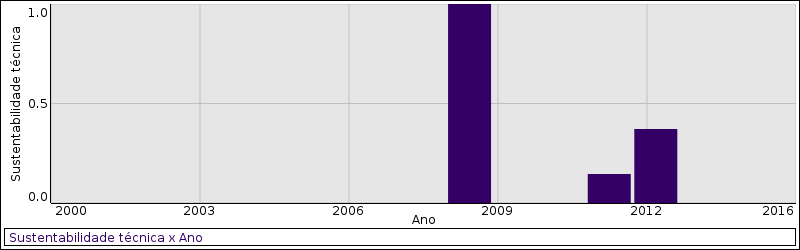
\includegraphics[scale=0.50]{imagens/softwares-charts/loopfrog.png}
  \caption{Sustentabilidade técnica do Loopfrog}
\end{figure}


\section{Lotrack}
\checkmark download
\checkmark código fonte


\begin{table}[H]
\caption{Versões lançadas e número de citações ao Lotrack por ano}
\centering
\begin{tabular}{| l | c | c | c | c | c |}
  \hline
  Ano & Versões & Peso da citação & Peso da autoria & Peso final & Sustentabilidade técnica \\
  \hline
            {\bf 2014}
          &
          
          &
          1.00
          &
          0.00
          &
          1.00
          &
            {\color{blue} 1.00}
          \\
\hline
            2015
          &
          
          &
          0.10
          &
          0.50
          &
          0.15
          &
            {\color{red} 0.15}
          \\
\hline
\end{tabular}
\end{table}

\begin{figure}[h]
  \center
  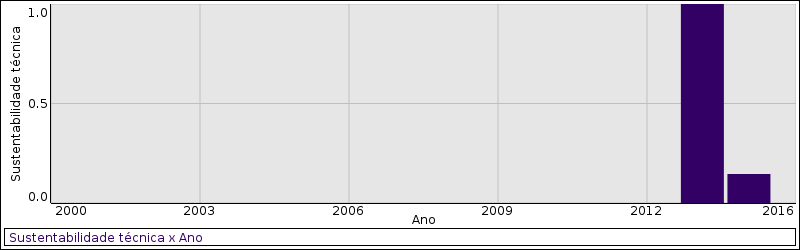
\includegraphics[scale=0.50]{imagens/softwares-charts/lotrack.png}
  \caption{Sustentabilidade técnica do Lotrack}
\end{figure}


\section{MPAnalyzer}
\checkmark download
\checkmark código fonte


\begin{table}[H]
\caption{Versões lançadas e número de citações ao MPAnalyzer por ano}
\centering
\begin{tabular}{| l | c | c | c | c | c |}
  \hline
  Ano & Versões & Peso da citação & Peso da autoria & Peso final & Sustentabilidade técnica \\
  \hline
            {\bf 2014}
          &
          
          &
          1.00
          &
          0.00
          &
          1.00
          &
            {\color{blue} 1.00}
          \\
\hline
\end{tabular}
\end{table}

\begin{figure}[h]
  \center
  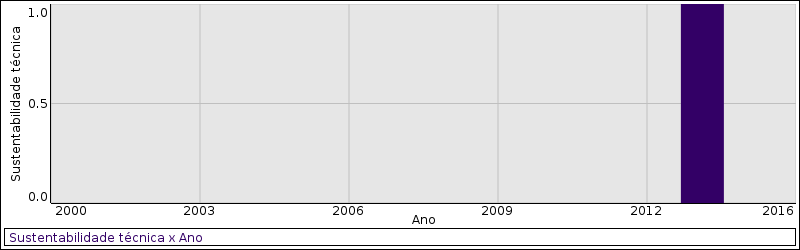
\includegraphics[scale=0.50]{imagens/softwares-charts/mpanalyzer.png}
  \caption{Sustentabilidade técnica do MPAnalyzer}
\end{figure}


\section{MSP}


\begin{table}[H]
\caption{Versões lançadas e número de citações ao MSP por ano}
\centering
\begin{tabular}{| l | c | c | c | c | c |}
  \hline
  Ano & Versões & Peso da citação & Peso da autoria & Peso final & Sustentabilidade técnica \\
  \hline
            2009
          &
          
          &
          0.10
            {\tiny MSP-GCC}
          &
          0.00
          &
          0.10
          &
            {\color{red} 0.10}
          \\
\hline
            {\bf 2010}
          &
          
          &
          1.00
          &
          0.50
          &
          1.00
          &
            {\color{blue} 1.00}
          \\
\hline
\end{tabular}
\end{table}

\begin{figure}[h]
  \center
  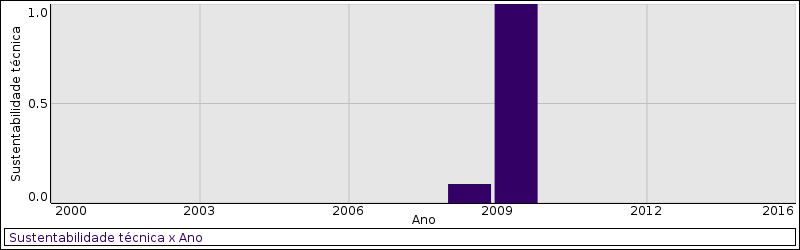
\includegraphics[scale=0.50]{imagens/softwares-charts/msp.png}
  \caption{Sustentabilidade técnica do MSP}
\end{figure}


\section{mygcc}
\checkmark download
\checkmark código fonte
\checkmark licença


\begin{table}[H]
\caption{Versões lançadas e número de citações ao mygcc por ano}
\centering
\begin{tabular}{| l | c | c | c | c | c |}
  \hline
  Ano & Versões & Peso da citação & Peso da autoria & Peso final & Sustentabilidade técnica \\
  \hline
            {\bf 2006}
          &
          
          &
          1.00
          &
          0.00
          &
          1.00
          &
            {\color{blue} 1.00}
          \\
            2006
          &
          
          &
          1.00
          &
          0.00
          &
          1.00
          &
          \\
\hline
            2008
          &
          
          &
          0.50
          &
          0.00
          &
          0.50
          &
            {\color{blue} 0.50}
          \\
\hline
            2009
          &
          
          &
          0.10
          &
          0.50
          &
          0.15
          &
            {\color{red} 0.15}
          \\
            2009
          &
          
          &
          0.10
          &
          0.50
          &
          0.15
          &
          \\
\hline
            2010
          &
          
          &
          0.25
          &
          0.50
          &
          0.38
          &
            {\color{red} 0.38}
          \\
\hline
            2014
          &
          
          &
          0.10
          &
          0.50
          &
          0.15
          &
            {\color{red} 0.15}
          \\
\hline
\end{tabular}
\end{table}

\begin{figure}[h]
  \center
  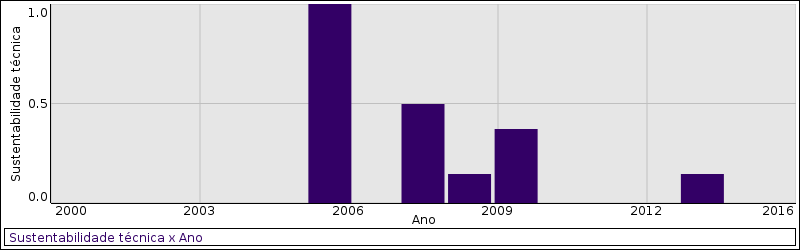
\includegraphics[scale=0.50]{imagens/softwares-charts/mygcc.png}
  \caption{Sustentabilidade técnica do mygcc}
\end{figure}


\section{PARSEWeb}


\begin{table}[H]
\caption{Versões lançadas e número de citações ao PARSEWeb por ano}
\centering
\begin{tabular}{| l | c | c | c | c | c |}
  \hline
  Ano & Versões & Peso da citação & Peso da autoria & Peso final & Sustentabilidade técnica \\
  \hline
            {\bf 2007}
          &
          
          &
          1.00
          &
          0.00
          &
          1.00
          &
            {\color{blue} 1.00}
          \\
\hline
            2008
          &
          
          &
          0.25
          &
          0.50
          &
          0.38
          &
            {\color{red} 0.38}
          \\
            2008
          &
          
          &
          0.10
          &
          0.00
          &
          0.10
          &
          \\
            2008
          &
          
          &
          0.10
          &
          0.50
          &
          0.15
          &
          \\
\hline
            2010
          &
          
          &
          0.10
          &
          0.50
          &
          0.15
          &
            {\color{red} 0.15}
          \\
\hline
            2011
          &
          
          &
          0.10
          &
          0.50
          &
          0.15
          &
            {\color{red} 0.15}
          \\
            2011
          &
          
          &
          0.10
          &
          0.50
          &
          0.15
          &
          \\
            2011
          &
          
          &
          0.10
          &
          0.50
          &
          0.15
          &
          \\
            2011
          &
          
          &
          0.10
          &
          0.50
          &
          0.15
          &
          \\
            2011
          &
          
          &
          0.10
          &
          0.50
          &
          0.15
          &
          \\
\hline
            2012
          &
          
          &
          0.10
          &
          0.50
          &
          0.15
          &
            {\color{red} 0.15}
          \\
            2012
          &
          
          &
          0.10
          &
          0.25
          &
          0.12
          &
          \\
            2012
          &
          
          &
          0.10
          &
          0.25
          &
          0.12
          &
          \\
            2012
          &
          
          &
          0.10
          &
          0.50
          &
          0.15
          &
          \\
            2012
          &
          
          &
          0.10
          &
          0.50
          &
          0.15
          &
          \\
            2012
          &
          
          &
          0.10
          &
          0.50
          &
          0.15
          &
          \\
\hline
            2013
          &
          
          &
          0.10
          &
          0.50
          &
          0.15
          &
            {\color{red} 0.15}
          \\
            2013
          &
          
          &
          0.10
          &
          0.50
          &
          0.15
          &
          \\
            2013
          &
          
          &
          0.10
          &
          0.50
          &
          0.15
          &
          \\
\hline
            2015
          &
          
          &
          0.10
          &
          0.25
          &
          0.12
          &
            {\color{red} 0.12}
          \\
            2015
          &
          
          &
          0.10
          &
          0.10
          &
          0.11
          &
          \\
\hline
            2016
          &
          
          &
          0.10
          &
          0.50
          &
          0.15
          &
            {\color{red} 0.15}
          \\
            2016
          &
          
          &
          0.10
          &
          0.50
          &
          0.15
          &
          \\
            2016
          &
          
          &
          0.10
          &
          0.25
          &
          0.12
          &
          \\
\hline
\end{tabular}
\end{table}

\begin{figure}[h]
  \center
  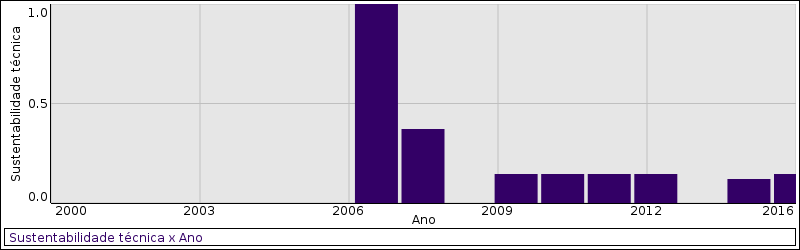
\includegraphics[scale=0.50]{imagens/softwares-charts/parseweb.png}
  \caption{Sustentabilidade técnica do PARSEWeb}
\end{figure}


\section{PAT - Puzzle-Based Automatic Testing}


\begin{table}[H]
\caption{Versões lançadas e número de citações ao PAT por ano}
\centering
\begin{tabular}{| l | c | c | c | c | c |}
  \hline
  Ano & Versões & Peso da citação & Peso da autoria & Peso final & Sustentabilidade técnica \\
  \hline
            {\bf 2012}
          &
          
          &
          1.00
          &
          0.00
          &
          1.00
          &
            {\color{blue} 1.00}
          \\
\hline
            2016
          &
          
          &
          0.10
          &
          0.50
          &
          0.15
          &
            {\color{red} 0.15}
          \\
\hline
\end{tabular}
\end{table}

\begin{figure}[h]
  \center
  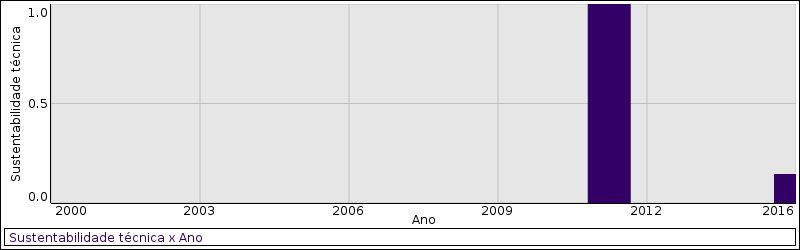
\includegraphics[scale=0.50]{imagens/softwares-charts/pat.png}
  \caption{Sustentabilidade técnica do PAT}
\end{figure}


\section{PHP AiR}
\checkmark download
\checkmark código fonte


\begin{table}[H]
\caption{Versões lançadas e número de citações ao PHP AiR por ano}
\centering
\begin{tabular}{| l | c | c | c | c | c |}
  \hline
  Ano & Versões & Peso da citação & Peso da autoria & Peso final & Sustentabilidade técnica \\
  \hline
        2011 & 1 & - & - & -
        &
          {\color{blue} 1.00}
        \\
\hline
        2012 & 1 & - & - & -
        &
          {\color{blue} 1.00}
        \\
\hline
            2014
          &
          2
          &
          0.10
          &
          0.00
          &
          0.10
          &
            {\color{blue} 1.00}
          \\
            {\bf 2014}
          &
          
          &
          1.00
          &
          0.00
          &
          1.00
          &
          \\
\hline
            2015
          &
          
          &
          0.25
          &
          0.25
          &
          0.31
          &
            {\color{blue} 0.62}
          \\
            2015
          &
          
          &
          0.50
          &
          0.00
          &
          0.50
          &
          \\
            2015
          &
          
          &
          0.25
          &
          0.25
          &
          0.31
          &
          \\
            2015
          &
          
          &
          0.50
          &
          0.25
          &
          0.62
          &
          \\
            2015
          &
          
          &
          0.25
          &
          0.25
          &
          0.31
          &
          \\
\hline
            2016
          &
          
          &
          0.25
          &
          0.10
          &
          0.28
          &
            {\color{red} 0.28}
          \\
\hline
            2017
          &
          
          &
          0.25
          &
          0.25
          &
          0.31
          &
            {\color{red} 0.31}
          \\
\hline
\end{tabular}
\end{table}

\begin{figure}[h]
  \center
  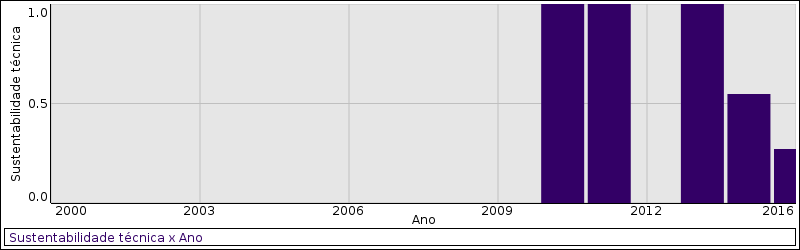
\includegraphics[scale=0.50]{imagens/softwares-charts/php-air.png}
  \caption{Sustentabilidade técnica do PHP AiR}
\end{figure}


\section{protopurity}
\checkmark download
\checkmark código fonte


\begin{table}[H]
\caption{Versões lançadas e número de citações ao protopurity por ano}
\centering
\begin{tabular}{| l | c | c | c | c | c |}
  \hline
  Ano & Versões & Peso da citação & Peso da autoria & Peso final & Sustentabilidade técnica \\
  \hline
            {\bf 2015}
          &
          
          &
          1.00
          &
          0.00
          &
          1.00
          &
            {\color{blue} 1.00}
          \\
\hline
\end{tabular}
\end{table}

\begin{figure}[h]
  \center
  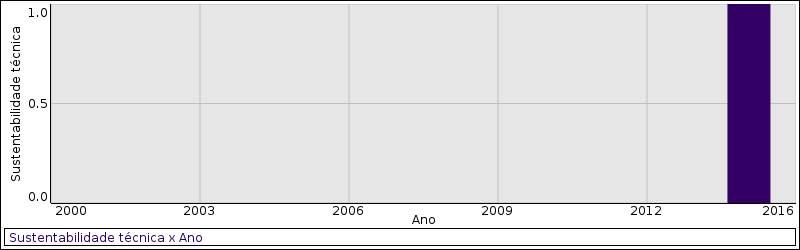
\includegraphics[scale=0.50]{imagens/softwares-charts/protopurity.png}
  \caption{Sustentabilidade técnica do protopurity}
\end{figure}


\section{Pseudogen}
\checkmark download
\checkmark código fonte


\begin{table}[H]
\caption{Versões lançadas e número de citações ao Pseudogen por ano}
\centering
\begin{tabular}{| l | c | c | c | c | c |}
  \hline
  Ano & Versões & Peso da citação & Peso da autoria & Peso final & Sustentabilidade técnica \\
  \hline
            {\bf 2015}
          &
          
          &
          1.00
          &
          0.00
          &
          1.00
          &
            {\color{blue} 1.00}
          \\
\hline
\end{tabular}
\end{table}

\begin{figure}[h]
  \center
  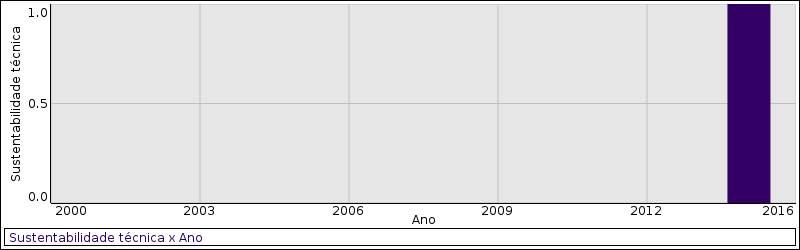
\includegraphics[scale=0.50]{imagens/softwares-charts/pseudogen.png}
  \caption{Sustentabilidade técnica do Pseudogen}
\end{figure}


\section{PtYasm}
\checkmark download
\checkmark código fonte


\begin{table}[H]
\caption{Versões lançadas e número de citações ao PtYasm por ano}
\centering
\begin{tabular}{| l | c | c | c | c | c |}
  \hline
  Ano & Versões & Peso da citação & Peso da autoria & Peso final & Sustentabilidade técnica \\
  \hline
            {\bf 2008}
          &
          
          &
          0.50
          &
          0.00
          &
          0.50
          &
            {\color{blue} 0.50}
          \\
            {\bf 2008}
          &
          
          &
          0.50
          &
          0.00
          &
          0.50
          &
          \\
\hline
\end{tabular}
\end{table}

\begin{figure}[h]
  \center
  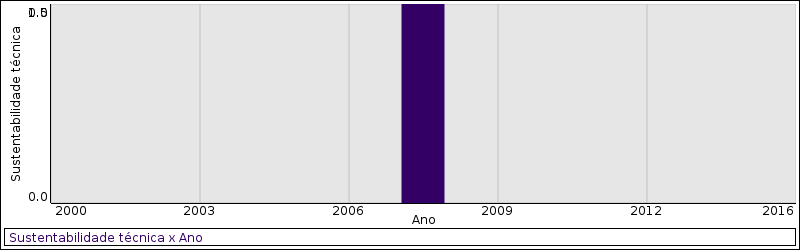
\includegraphics[scale=0.50]{imagens/softwares-charts/ptyasm.png}
  \caption{Sustentabilidade técnica do PtYasm}
\end{figure}


\section{PuMoC}


\begin{table}[H]
\caption{Versões lançadas e número de citações ao PuMoC por ano}
\centering
\begin{tabular}{| l | c | c | c | c | c |}
  \hline
  Ano & Versões & Peso da citação & Peso da autoria & Peso final & Sustentabilidade técnica \\
  \hline
            {\bf 2012}
          &
          
          &
          1.00
          &
          0.00
          &
          1.00
          &
            {\color{blue} 1.00}
          \\
\hline
            2013
          &
          
          &
          0.10
          &
          0.10
          &
          0.11
          &
            {\color{red} 0.11}
          \\
\hline
\end{tabular}
\end{table}

\begin{figure}[h]
  \center
  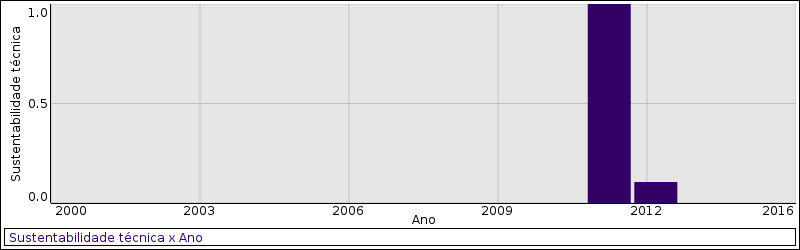
\includegraphics[scale=0.50]{imagens/softwares-charts/pumoc.png}
  \caption{Sustentabilidade técnica do PuMoC}
\end{figure}


\section{PYTHIA}


\begin{table}[H]
\caption{Versões lançadas e número de citações ao PYTHIA por ano}
\centering
\begin{tabular}{| l | c | c | c | c | c |}
  \hline
  Ano & Versões & Peso da citação & Peso da autoria & Peso final & Sustentabilidade técnica \\
  \hline
            {\bf 2013}
          &
          
          &
          1.00
          &
          0.00
          &
          1.00
          &
            {\color{blue} 1.00}
          \\
\hline
            2014
          &
          
          &
          0.50
          &
          0.10
          &
          0.55
          &
            {\color{blue} 0.55}
          \\
\hline
\end{tabular}
\end{table}

\begin{figure}[h]
  \center
  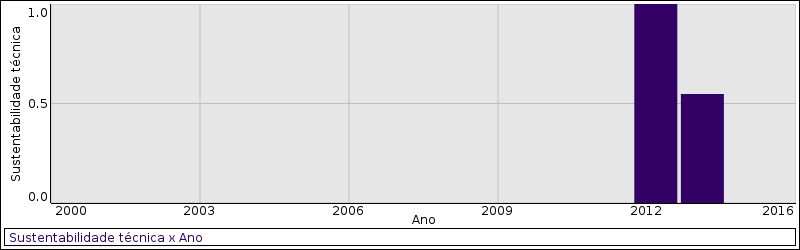
\includegraphics[scale=0.50]{imagens/softwares-charts/pythia.png}
  \caption{Sustentabilidade técnica do PYTHIA}
\end{figure}


\section{ReAssert}
\checkmark download
\checkmark código fonte
\checkmark licença


\begin{table}[H]
\caption{Versões lançadas e número de citações ao ReAssert por ano}
\centering
\begin{tabular}{| l | c | c | c | c | c |}
  \hline
  Ano & Versões & Peso da citação & Peso da autoria & Peso final & Sustentabilidade técnica \\
  \hline
            {\bf 2009}
          &
          2
          &
          1.00
          &
          0.00
          &
          1.00
          &
            {\color{blue} 1.00}
          \\
\hline
            2010
          &
          3
          &
          0.25
          &
          0.25
          &
          0.31
          &
            {\color{blue} 1.00}
          \\
\hline
            2011
          &
          
          &
          0.10
          &
          0.00
          &
          0.10
          &
            {\color{red} 0.25}
          \\
            2011
          &
          
          &
          0.25
          &
          0.00
          &
          0.25
          &
          \\
            2011
          &
          
          &
          0.10
          &
          0.00
          &
          0.10
          &
          \\
            2011
          &
          
          &
          0.10
          &
          0.00
          &
          0.10
          &
          \\
\hline
            2012
          &
          
          &
          0.25
          &
          0.25
          &
          0.31
          &
            {\color{red} 0.31}
          \\
            2012
          &
          
          &
          0.10
          &
          0.25
          &
          0.12
          &
          \\
            2012
          &
          
          &
          0.10
          &
          0.25
          &
          0.12
          &
          \\
\hline
            2013
          &
          
          &
          0.10
          &
          0.50
          &
          0.15
          &
            {\color{red} 0.15}
          \\
            2013
          &
          
          &
          0.10
          &
          0.50
          &
          0.15
          &
          \\
\hline
            2016
          &
          
          &
          0.10
          &
          0.25
          &
          0.12
          &
            {\color{red} 0.12}
          \\
            2016
          &
          
          &
          0.10
            {\tiny COOPE}
          &
          0.25
          &
          0.12
          &
          \\
\hline
\end{tabular}
\end{table}

\begin{figure}[h]
  \center
  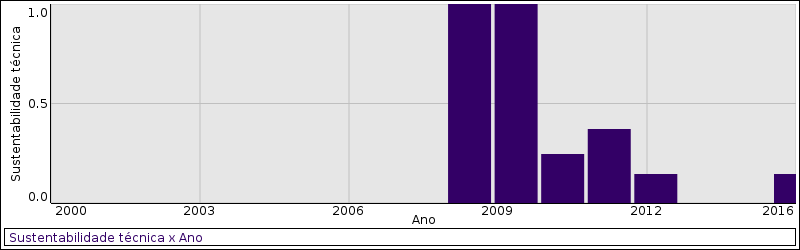
\includegraphics[scale=0.50]{imagens/softwares-charts/reassert.png}
  \caption{Sustentabilidade técnica do ReAssert}
\end{figure}


\section{Rêve}


\begin{table}[H]
\caption{Versões lançadas e número de citações ao Rêve por ano}
\centering
\begin{tabular}{| l | c | c | c | c | c |}
  \hline
  Ano & Versões & Peso da citação & Peso da autoria & Peso final & Sustentabilidade técnica \\
  \hline
            {\bf 2014}
          &
          
          &
          1.00
          &
          0.00
          &
          1.00
          &
            {\color{blue} 1.00}
          \\
\hline
\end{tabular}
\end{table}

\begin{figure}[h]
  \center
  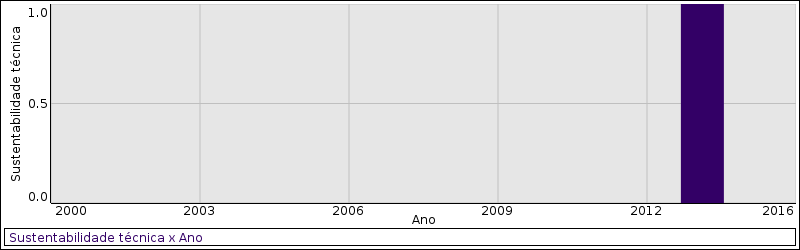
\includegraphics[scale=0.50]{imagens/softwares-charts/reve.png}
  \caption{Sustentabilidade técnica do Rêve}
\end{figure}


\section{RRFinder}


\begin{table}[H]
\caption{Versões lançadas e número de citações ao RRFinder por ano}
\centering
\begin{tabular}{| l | c | c | c | c | c |}
  \hline
  Ano & Versões & Peso da citação & Peso da autoria & Peso final & Sustentabilidade técnica \\
  \hline
            {\bf 2011}
          &
          
          &
          1.00
          &
          0.00
          &
          1.00
          &
            {\color{blue} 1.00}
          \\
\hline
            2014
          &
          
          &
          0.10
          &
          0.50
          &
          0.15
          &
            {\color{red} 0.15}
          \\
\hline
            2015
          &
          
          &
          0.10
          &
          0.50
          &
          0.15
          &
            {\color{red} 0.15}
          \\
\hline
\end{tabular}
\end{table}

\begin{figure}[h]
  \center
  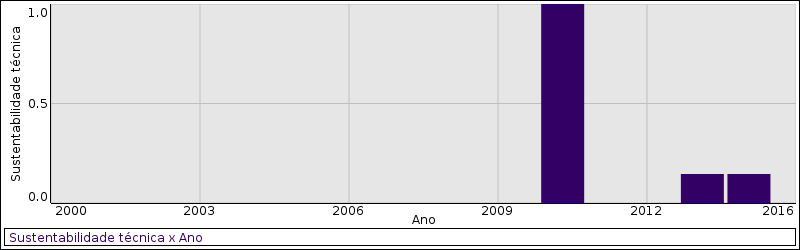
\includegraphics[scale=0.50]{imagens/softwares-charts/rrfinder.png}
  \caption{Sustentabilidade técnica do RRFinder}
\end{figure}


\section{Sapid/XML}


\begin{table}[H]
\caption{Versões lançadas e número de citações ao Sapid/XML por ano}
\centering
\begin{tabular}{| l | c | c | c | c | c |}
  \hline
  Ano & Versões & Peso da citação & Peso da autoria & Peso final & Sustentabilidade técnica \\
  \hline
            {\bf 2004}
          &
          
          &
          1.00
          &
          0.00
          &
          1.00
          &
            {\color{blue} 1.00}
          \\
\hline
            2005
          &
          
          &
          0.25
          &
          0.00
          &
          0.25
          &
            {\color{blue} 0.55}
          \\
            2005
          &
          
          &
          0.50
          &
          0.10
          &
          0.55
          &
          \\
\hline
            2006
          &
          
          &
          0.25
          &
          0.10
          &
          0.28
          &
            {\color{red} 0.28}
          \\
\hline
            2012
          &
          
          &
          0.10
          &
          0.50
          &
          0.15
          &
            {\color{red} 0.15}
          \\
\hline
\end{tabular}
\end{table}

\begin{figure}[h]
  \center
  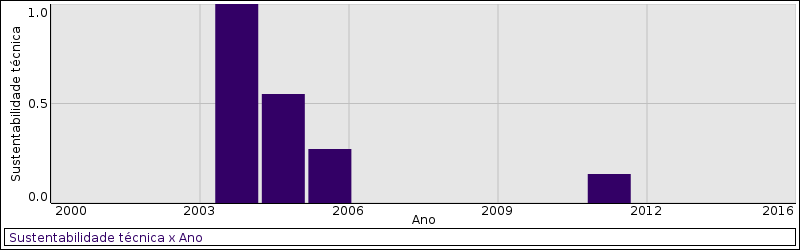
\includegraphics[scale=0.50]{imagens/softwares-charts/sapid-xml.png}
  \caption{Sustentabilidade técnica do Sapid/XML}
\end{figure}


\section{Sonar Qube Plug-in}
\checkmark download
\checkmark código fonte
\checkmark licença


\begin{table}[H]
\caption{Versões lançadas e número de citações ao Sonar Qube Plug-in por ano}
\centering
\begin{tabular}{| l | c | c | c | c | c |}
  \hline
  Ano & Versões & Peso da citação & Peso da autoria & Peso final & Sustentabilidade técnica \\
  \hline
            {\bf 2014}
          &
          
          &
          1.00
          &
          0.00
          &
          1.00
          &
            {\color{blue} 1.00}
          \\
\hline
        2015 & 3 & - & - & -
        &
          {\color{blue} 1.00}
        \\
\hline
        2016 & 1 & - & - & -
        &
          {\color{blue} 1.00}
        \\
\hline
\end{tabular}
\end{table}

\begin{figure}[h]
  \center
  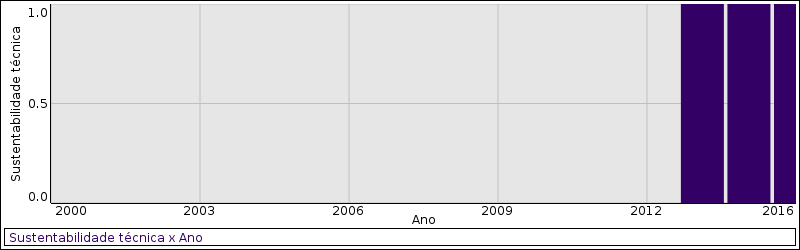
\includegraphics[scale=0.50]{imagens/softwares-charts/sonarqube-plugin.png}
  \caption{Sustentabilidade técnica do Sonar Qube Plug-in}
\end{figure}


\section{SPARTA - Static Program Analysis for Reliable Trusted Apps}
\checkmark download
\checkmark código fonte


\begin{table}[H]
\caption{Versões lançadas e número de citações ao SPARTA por ano}
\centering
\begin{tabular}{| l | c | c | c | c | c |}
  \hline
  Ano & Versões & Peso da citação & Peso da autoria & Peso final & Sustentabilidade técnica \\
  \hline
            2002
          &
          
          &
          0.25
          &
          0.00
          &
          0.25
          &
            {\color{red} 0.25}
          \\
\hline
        2012 & 1 & - & - & -
        &
          {\color{blue} 1.00}
        \\
\hline
        2013 & 7 & - & - & -
        &
          {\color{blue} 1.00}
        \\
\hline
        2014 & 4 & - & - & -
        &
          {\color{blue} 1.00}
        \\
\hline
            {\bf 2015}
          &
          1
          &
          1.00
          &
          0.50
          &
          1.00
          &
            {\color{blue} 1.00}
          \\
\hline
        2016 & 1 & - & - & -
        &
          {\color{blue} 1.00}
        \\
\hline
            2017
          &
          
          &
          0.25
          &
          0.50
          &
          0.38
          &
            {\color{red} 0.38}
          \\
            2017
          &
          
          &
          0.10
          &
          0.50
          &
          0.15
          &
          \\
\hline
\end{tabular}
\end{table}

\begin{figure}[h]
  \center
  \includegraphics[scale=0.50]{imagens/softwares-charts/sparta.png}
  \caption{Sustentabilidade técnica do SPARTA}
\end{figure}


\section{srcML}
\checkmark download
\checkmark código fonte
\checkmark licença


\begin{table}[H]
\caption{Versões lançadas e número de citações ao srcML por ano}
\centering
\begin{tabular}{| l | c | c | c | c | c |}
  \hline
  Ano & Versões & Peso da citação & Peso da autoria & Peso final & Sustentabilidade técnica \\
  \hline
            2002
          &
          
          &
          0.10
          &
          0.00
          &
          0.10
          &
            {\color{red} 0.10}
          \\
\hline
            2003
          &
          
          &
          0.10
          &
          0.50
          &
          0.15
          &
            {\color{red} 0.15}
          \\
\hline
            2004
          &
          
          &
          0.25
          &
          0.50
          &
          0.38
          &
            {\color{red} 0.38}
          \\
            2004
          &
          
          &
          0.25
          &
          0.50
          &
          0.38
          &
          \\
            2004
          &
          
          &
          0.10
          &
          0.50
          &
          0.15
          &
          \\
\hline
            2005
          &
          
          &
          0.25
          &
          0.50
          &
          0.38
          &
            {\color{red} 0.38}
          \\
            2005
          &
          
          &
          0.10
          &
          0.50
          &
          0.15
          &
          \\
            2005
          &
          
          &
          0.10
          &
          0.25
          &
          0.12
          &
          \\
\hline
            2007
          &
          
          &
          0.10
          &
          0.25
          &
          0.12
          &
            {\color{red} 0.12}
          \\
\hline
            2008
          &
          
          &
          0.10
          &
          0.25
          &
          0.12
          &
            {\color{red} 0.12}
          \\
\hline
            2009
          &
          
          &
          0.25
          &
          0.50
          &
          0.38
          &
            {\color{red} 0.38}
          \\
            2009
          &
          
          &
          0.10
          &
          0.50
          &
          0.15
          &
          \\
            2009
          &
          
          &
          0.10
          &
          0.50
          &
          0.15
          &
          \\
\hline
            2010
          &
          
          &
          0.25
          &
          0.25
          &
          0.31
          &
            {\color{red} 0.31}
          \\
\hline
            2011
          &
          3
          &
          0.25
          &
          0.25
          &
          0.31
          &
            {\color{blue} 1.00}
          \\
            2011
          &
          
          &
          0.25
          &
          0.50
          &
          0.38
          &
          \\
            {\bf 2011}
          &
          
          &
          1.00
          &
          0.25
          &
          1.00
          &
          \\
\hline
            2012
          &
          5
          &
          0.25
          &
          0.25
          &
          0.31
          &
            {\color{blue} 1.00}
          \\
            2012
          &
          
          &
          0.25
          &
          0.25
          &
          0.31
          &
          \\
            2012
          &
          
          &
          0.25
          &
          0.25
          &
          0.31
          &
          \\
\hline
            2013
          &
          1
          &
          0.25
          &
          0.25
          &
          0.31
          &
            {\color{blue} 1.00}
          \\
            2013
          &
          
          &
          0.25
          &
          0.50
          &
          0.38
          &
          \\
            2013
          &
          
          &
          0.10
          &
          0.25
          &
          0.12
          &
          \\
            2013
          &
          
          &
          0.10
          &
          0.25
          &
          0.12
          &
          \\
\hline
            2014
          &
          4
          &
          0.25
          &
          0.50
          &
          0.38
          &
            {\color{blue} 1.00}
          \\
            2014
          &
          
          &
          0.25
          &
          0.25
          &
          0.31
          &
          \\
            2014
          &
          
          &
          0.25
          &
          0.50
          &
          0.38
          &
          \\
            2014
          &
          
          &
          0.25
          &
          0.50
          &
          0.38
          &
          \\
\hline
            2015
          &
          1
          &
          0.10
          &
          0.25
          &
          0.12
          &
            {\color{blue} 1.00}
          \\
            2015
          &
          
          &
          0.10
          &
          0.25
          &
          0.12
          &
          \\
            2015
          &
          
          &
          0.25
          &
          0.25
          &
          0.31
          &
          \\
\hline
            2016
          &
          
          &
          0.25
          &
          0.25
          &
          0.31
          &
            {\color{blue} 0.62}
          \\
            2016
          &
          
          &
          0.50
          &
          0.25
          &
          0.62
          &
          \\
            2016
          &
          
          &
          0.25
          &
          0.25
          &
          0.31
          &
          \\
            2016
          &
          
          &
          0.25
          &
          0.25
          &
          0.31
          &
          \\
            2016
          &
          
          &
          0.25
          &
          0.25
          &
          0.31
          &
          \\
            2016
          &
          
          &
          0.50
          &
          0.25
          &
          0.62
          &
          \\
\hline
            2017
          &
          
          &
          0.25
          &
          0.25
          &
          0.31
          &
            {\color{red} 0.38}
          \\
            2017
          &
          
          &
          0.25
          &
          0.50
          &
          0.38
          &
          \\
            2017
          &
          
          &
          0.10
            {\tiny srcQL}
          &
          0.25
          &
          0.12
          &
          \\
\hline
\end{tabular}
\end{table}

\begin{figure}[h]
  \center
  \includegraphics[scale=0.50]{imagens/softwares-charts/srcml.png}
  \caption{Sustentabilidade técnica do srcML}
\end{figure}


\section{SWAT - Search based Web Application Tester}


\begin{table}[H]
\caption{Versões lançadas e número de citações ao SWAT por ano}
\centering
\begin{tabular}{| l | c | c | c | c | c |}
  \hline
  Ano & Versões & Peso da citação & Peso da autoria & Peso final & Sustentabilidade técnica \\
  \hline
            {\bf 2011}
          &
          
          &
          1.00
          &
          0.00
          &
          1.00
          &
            {\color{blue} 1.00}
          \\
\hline
            2012
          &
          
          &
          0.25
          &
          0.10
          &
          0.28
          &
            {\color{red} 0.28}
          \\
\hline
            2013
          &
          
          &
          0.10
          &
          0.50
          &
          0.15
          &
            {\color{red} 0.15}
          \\
\hline
            2014
          &
          
          &
          0.25
          &
          0.10
          &
          0.28
          &
            {\color{red} 0.28}
          \\
\hline
\end{tabular}
\end{table}

\begin{figure}[h]
  \center
  \includegraphics[scale=0.50]{imagens/softwares-charts/swat.png}
  \caption{Sustentabilidade técnica do SWAT}
\end{figure}


\section{TACLE - Type Analysis and CalL graph construction for Eclipse}
\checkmark download
\checkmark código fonte


\begin{table}[H]
\caption{Versões lançadas e número de citações ao TACLE por ano}
\centering
\begin{tabular}{| l | c | c | c | c | c |}
  \hline
  Ano & Versões & Peso da citação & Peso da autoria & Peso final & Sustentabilidade técnica \\
  \hline
            2005
          &
          
          &
          0.25
          &
          0.00
          &
          0.25
          &
            {\color{red} 0.25}
          \\
\hline
            {\bf 2006}
          &
          
          &
          1.00
          &
          0.10
          &
          1.00
          &
            {\color{blue} 1.00}
          \\
            2006
          &
          
          &
          0.10
          &
          0.10
          &
          0.11
          &
          \\
\hline
\end{tabular}
\end{table}

\begin{figure}[h]
  \center
  \includegraphics[scale=0.50]{imagens/softwares-charts/tacle.png}
  \caption{Sustentabilidade técnica do TACLE}
\end{figure}


\section{TEBA}
\checkmark download
\checkmark código fonte


\begin{table}[H]
\caption{Versões lançadas e número de citações ao TEBA por ano}
\centering
\begin{tabular}{| l | c | c | c | c | c |}
  \hline
  Ano & Versões & Peso da citação & Peso da autoria & Peso final & Sustentabilidade técnica \\
  \hline
        2010 & 1 & - & - & -
        &
          {\color{blue} 1.00}
        \\
\hline
        2011 & 5 & - & - & -
        &
          {\color{blue} 1.00}
        \\
\hline
        2012 & 4 & - & - & -
        &
          {\color{blue} 1.00}
        \\
\hline
        2013 & 5 & - & - & -
        &
          {\color{blue} 1.00}
        \\
\hline
            {\bf 2014}
          &
          5
          &
          1.00
          &
          0.00
          &
          1.00
          &
            {\color{blue} 1.00}
          \\
\hline
        2016 & 1 & - & - & -
        &
          {\color{blue} 1.00}
        \\
\hline
\end{tabular}
\end{table}

\begin{figure}[h]
  \center
  \includegraphics[scale=0.50]{imagens/softwares-charts/teba.png}
  \caption{Sustentabilidade técnica do TEBA}
\end{figure}


\section{TestEra}


\begin{table}[H]
\caption{Versões lançadas e número de citações ao TestEra por ano}
\centering
\begin{tabular}{| l | c | c | c | c | c |}
  \hline
  Ano & Versões & Peso da citação & Peso da autoria & Peso final & Sustentabilidade técnica \\
  \hline
            {\bf 2001}
          &
          
          &
          1.00
          &
          0.00
          &
          1.00
          &
            {\color{blue} 1.00}
          \\
\hline
            2002
          &
          
          &
          0.10
          &
          0.00
          &
          0.10
          &
            {\color{red} 0.10}
          \\
\hline
            2004
          &
          
          &
          0.10
          &
          0.25
          &
          0.12
          &
            {\color{red} 0.12}
          \\
\hline
            2005
          &
          
          &
          0.10
          &
          0.25
          &
          0.12
          &
            {\color{red} 0.31}
          \\
            2005
          &
          
          &
          0.25
          &
          0.25
          &
          0.31
          &
          \\
\hline
            2006
          &
          
          &
          0.10
            {\tiny aDeryaft compatible}
          &
          0.25
          &
          0.12
          &
            {\color{red} 0.12}
          \\
\hline
            2007
          &
          
          &
          0.25
          &
          0.25
          &
          0.31
          &
            {\color{red} 0.31}
          \\
            2007
          &
          
          &
          0.25
          &
          0.25
          &
          0.31
          &
          \\
            2007
          &
          
          &
          0.10
          &
          0.25
          &
          0.12
          &
          \\
            2007
          &
          
          &
          0.25
          &
          0.25
          &
          0.31
          &
          \\
\hline
            2008
          &
          
          &
          0.10
          &
          0.25
          &
          0.12
          &
            {\color{red} 0.31}
          \\
            2008
          &
          
          &
          0.25
          &
          0.25
          &
          0.31
          &
          \\
\hline
            2009
          &
          
          &
          0.10
          &
          0.25
          &
          0.12
          &
            {\color{red} 0.12}
          \\
            2009
          &
          
          &
          0.10
          &
          0.25
          &
          0.12
          &
          \\
\hline
            2010
          &
          
          &
          0.10
          &
          0.25
          &
          0.12
          &
            {\color{red} 0.12}
          \\
            2010
          &
          
          &
          0.10
          &
          0.25
          &
          0.12
          &
          \\
\hline
            2011
          &
          
          &
          0.10
          &
          0.10
          &
          0.11
          &
            {\color{red} 0.12}
          \\
            2011
          &
          
          &
          0.10
          &
          0.25
          &
          0.12
          &
          \\
            2011
          &
          
          &
          0.10
          &
          0.25
          &
          0.12
          &
          \\
\hline
            2012
          &
          
          &
          0.10
          &
          0.10
          &
          0.11
          &
            {\color{red} 0.12}
          \\
            2012
          &
          
          &
          0.10
          &
          0.25
          &
          0.12
          &
          \\
\hline
            2013
          &
          
          &
          0.10
          &
          0.50
          &
          0.15
          &
            {\color{red} 0.15}
          \\
\hline
            2014
          &
          
          &
          0.10
          &
          0.50
          &
          0.15
          &
            {\color{red} 0.15}
          \\
\hline
\end{tabular}
\end{table}

\begin{figure}[h]
  \center
  \includegraphics[scale=0.50]{imagens/softwares-charts/testera.png}
  \caption{Sustentabilidade técnica do TestEra}
\end{figure}


\section{Vdiff}


\begin{table}[H]
\caption{Versões lançadas e número de citações ao Vdiff por ano}
\centering
\begin{tabular}{| l | c | c | c | c | c |}
  \hline
  Ano & Versões & Peso da citação & Peso da autoria & Peso final & Sustentabilidade técnica \\
  \hline
            {\bf 2010}
          &
          
          &
          1.00
          &
          0.00
          &
          1.00
          &
            {\color{blue} 1.00}
          \\
\hline
            2011
          &
          
          &
          0.10
          &
          0.50
          &
          0.15
          &
            {\color{red} 0.15}
          \\
            2011
          &
          
          &
          0.10
          &
          0.50
          &
          0.15
          &
          \\
\hline
            2015
          &
          
          &
          0.10
          &
          0.50
          &
          0.15
          &
            {\color{red} 0.15}
          \\
\hline
            2016
          &
          
          &
          0.10
          &
          0.50
          &
          0.15
          &
            {\color{red} 0.15}
          \\
\hline
\end{tabular}
\end{table}

\begin{figure}[h]
  \center
  \includegraphics[scale=0.50]{imagens/softwares-charts/vdiff.png}
  \caption{Sustentabilidade técnica do Vdiff}
\end{figure}


\section{WALA}
\checkmark download
\checkmark código fonte
\checkmark licença


\begin{table}[H]
\caption{Versões lançadas e número de citações ao WALA por ano}
\centering
\begin{tabular}{| l | c | c | c | c | c |}
  \hline
  Ano & Versões & Peso da citação & Peso da autoria & Peso final & Sustentabilidade técnica \\
  \hline
        2006 & 1 & - & - & -
        &
          {\color{blue} 1.00}
        \\
\hline
        2007 & 6 & - & - & -
        &
          {\color{blue} 1.00}
        \\
\hline
            2008
          &
          4
          &
          0.25
          &
          0.00
          &
          0.25
          &
            {\color{blue} 1.00}
          \\
\hline
            2009
          &
          6
          &
          0.25
          &
          0.50
          &
          0.38
          &
            {\color{blue} 1.00}
          \\
\hline
            {\bf 2010}
          &
          4
          &
          1.00
          &
          0.25
          &
          1.00
          &
            {\color{blue} 1.00}
          \\
\hline
            2011
          &
          3
          &
          0.25
          &
          0.50
          &
          0.38
          &
            {\color{blue} 1.00}
          \\
\hline
            2012
          &
          2
          &
          0.25
          &
          0.50
          &
          0.38
          &
            {\color{blue} 1.00}
          \\
            2012
          &
          
          &
          0.10
          &
          0.50
          &
          0.15
          &
          \\
\hline
            2013
          &
          4
          &
          0.10
          &
          0.25
          &
          0.12
          &
            {\color{blue} 1.00}
          \\
\hline
        2015 & 2 & - & - & -
        &
          {\color{blue} 1.00}
        \\
\hline
            2016
          &
          1
          &
          0.10
          &
          0.25
          &
          0.12
          &
            {\color{blue} 1.00}
          \\
            2016
          &
          
          &
          0.25
          &
          0.25
          &
          0.31
          &
          \\
            2016
          &
          
          &
          0.10
          &
          0.25
          &
          0.12
          &
          \\
\hline
            2017
          &
          4
          &
          0.10
          &
          0.50
          &
          0.15
          &
            {\color{blue} 1.00}
          \\
\hline
\end{tabular}
\end{table}

\begin{figure}[h]
  \center
  \includegraphics[scale=0.50]{imagens/softwares-charts/wala.png}
  \caption{Sustentabilidade técnica do WALA}
\end{figure}


\section{Wrangler}
\checkmark download
\checkmark código fonte
\checkmark licença


\begin{table}[H]
\caption{Versões lançadas e número de citações ao Wrangler por ano}
\centering
\begin{tabular}{| l | c | c | c | c | c |}
  \hline
  Ano & Versões & Peso da citação & Peso da autoria & Peso final & Sustentabilidade técnica \\
  \hline
            2006
          &
          
          &
          0.25
          &
          0.00
          &
          0.25
          &
            {\color{red} 0.25}
          \\
\hline
            2008
          &
          
          &
          0.10
          &
          0.00
          &
          0.10
          &
            {\color{red} 0.25}
          \\
            2008
          &
          
          &
          0.25
          &
          0.00
          &
          0.25
          &
          \\
            2008
          &
          
          &
          0.10
          &
          0.00
          &
          0.10
          &
          \\
            2008
          &
          
          &
          0.10
          &
          0.00
          &
          0.10
          &
          \\
\hline
            2009
          &
          
          &
          0.10
          &
          0.25
          &
          0.12
          &
            {\color{blue} 0.62}
          \\
            2009
          &
          
          &
          0.25
          &
          0.25
          &
          0.31
          &
          \\
            2009
          &
          
          &
          0.25
          &
          0.25
          &
          0.31
          &
          \\
            2009
          &
          
          &
          0.50
          &
          0.25
          &
          0.62
          &
          \\
\hline
            2010
          &
          
          &
          0.10
          &
          0.25
          &
          0.12
          &
            {\color{blue} 1.00}
          \\
            2010
          &
          
          &
          0.10
          &
          0.50
          &
          0.15
          &
          \\
            2010
          &
          
          &
          0.10
          &
          0.25
          &
          0.12
          &
          \\
            2010
          &
          
          &
          0.25
          &
          0.25
          &
          0.31
          &
          \\
            {\bf 2010}
          &
          
          &
          1.00
          &
          0.25
          &
          1.00
          &
          \\
\hline
            2011
          &
          
          &
          0.50
          &
          0.10
          &
          0.55
          &
            {\color{blue} 0.55}
          \\
\hline
            2012
          &
          
          &
          0.10
          &
          0.50
          &
          0.15
          &
            {\color{blue} 0.62}
          \\
            2012
          &
          
          &
          0.50
          &
          0.25
          &
          0.62
          &
          \\
            2012
          &
          
          &
          0.50
          &
          0.25
          &
          0.62
          &
          \\
            2012
          &
          
          &
          0.10
          &
          0.25
          &
          0.12
          &
          \\
            2012
          &
          
          &
          0.10
          &
          0.25
          &
          0.12
          &
          \\
\hline
            2013
          &
          1
          &
          0.10
          &
          0.50
          &
          0.15
          &
            {\color{blue} 1.00}
          \\
            2013
          &
          
          &
          0.25
          &
          0.25
          &
          0.31
          &
          \\
            2013
          &
          
          &
          0.25
          &
          0.25
          &
          0.31
          &
          \\
\hline
            2014
          &
          1
          &
          0.50
          &
          0.25
          &
          0.62
          &
            {\color{blue} 1.00}
          \\
            2014
          &
          
          &
          0.50
          &
          0.25
          &
          0.62
          &
          \\
            2014
          &
          
          &
          0.10
          &
          0.25
          &
          0.12
          &
          \\
            2014
          &
          
          &
          0.10
          &
          0.25
          &
          0.12
          &
          \\
\hline
            2015
          &
          1
          &
          0.10
          &
          0.25
          &
          0.12
          &
            {\color{blue} 1.00}
          \\
            2015
          &
          
          &
          0.25
          &
          0.10
          &
          0.28
          &
          \\
\hline
            2016
          &
          
          &
          0.25
          &
          0.50
          &
          0.38
          &
            {\color{red} 0.38}
          \\
            2016
          &
          
          &
          0.25
          &
          0.25
          &
          0.31
          &
          \\
            2016
          &
          
          &
          0.10
          &
          0.50
          &
          0.15
          &
          \\
\hline
            2017
          &
          
          &
          0.10
          &
          0.25
          &
          0.12
          &
            {\color{red} 0.12}
          \\
\hline
\end{tabular}
\end{table}

\begin{figure}[h]
  \center
  \includegraphics[scale=0.50]{imagens/softwares-charts/wrangler.png}
  \caption{Sustentabilidade técnica do Wrangler}
\end{figure}


\section{XOgastan}


\begin{table}[H]
\caption{Versões lançadas e número de citações ao XOgastan por ano}
\centering
\begin{tabular}{| l | c | c | c | c | c |}
  \hline
  Ano & Versões & Peso da citação & Peso da autoria & Peso final & Sustentabilidade técnica \\
  \hline
            {\bf 2003}
          &
          
          &
          1.00
          &
          0.00
          &
          1.00
          &
            {\color{blue} 1.00}
          \\
\hline
            2004
          &
          
          &
          0.10
          &
          0.50
          &
          0.15
          &
            {\color{red} 0.15}
          \\
\hline
            2006
          &
          
          &
          0.10
          &
          0.50
          &
          0.15
          &
            {\color{red} 0.15}
          \\
\hline
            2008
          &
          
          &
          0.10
          &
          0.50
          &
          0.15
          &
            {\color{red} 0.15}
          \\
\hline
            2011
          &
          
          &
          0.10
          &
          0.50
          &
          0.15
          &
            {\color{red} 0.15}
          \\
\hline
\end{tabular}
\end{table}

\begin{figure}[h]
  \center
  \includegraphics[scale=0.50]{imagens/softwares-charts/xogastan.png}
  \caption{Sustentabilidade técnica do XOgastan}
\end{figure}



